\documentclass[12pt, oneside]{book}
\usepackage[utf8]{inputenc}
\usepackage{import}
\usepackage[font=footnotesize,labelfont=bf]{caption}
\usepackage{example}
\usepackage{makeidx}
\usepackage{fancyhdr}
\usepackage{amsmath}
\usepackage{hanging}
\usepackage{bm}
\usepackage{pdflscape}
\usepackage{booktabs}
\usepackage{multirow}
\usepackage{float}
\usepackage{subcaption}
\usepackage{graphicx}
\usepackage[a4paper,width=150mm,top=30mm,bottom=30mm,bindingoffset=6mm]{geometry}
\usepackage{setspace}

\usepackage{chngcntr}
\counterwithout{equation}{chapter} % continuous equation numbering
\counterwithout{figure}{chapter}    %continuous figure numbering
\counterwithout{table}{chapter}     %continuous table numbering

\graphicspath{ {images/} }
\pagestyle{fancy}
\setlength{\parskip}{1em}

\author{Prithvi Thakur}
\date{2015-16}

\begin{document}
\renewcommand{\baselinestretch}{1.0}
\begin{titlepage}
    \begin{center}
        \vspace*{1cm}
        
        \Huge
        \textbf{NEW METHODS FOR PALEOSTRESS ANALYSIS FROM FAULT-SLIP DATA}
        
        \vspace{0.5cm}
        
        \Large
        \textsc{A Dissertation}\\
        \vspace{0.5cm}
        \normalsize
        \emph{Submitted in partial fulfillment of the}\\ 
        \emph{requirements for the award of the degree}\\
        \emph{of}\\
        \textsc{Integrated Master of Technology}\\
        \emph{in}\\
        \textsc{Geological Technology}
        \vspace{1.5cm}
        
        By\\
        \textbf{Prithvi Thakur}
        
        
        \vspace{0.8cm}
        
        
\includegraphics[width=0.4\textwidth]{logo}
        
        \vspace{0.5cm}
        Department of Earth Sciences\\
        Indian Institute of Technology Roorkee\\
        Roorkee- 247667 (India)\\
        May, 2016
        
    \end{center}
\end{titlepage}

\frontmatter

\chapter{Declaration of Authorship}
 \textit{I hereby solemnly declare the work presented in this dissertation, entitled \textbf{"New methods for paleostress analysis from fault-slip data"} in partial fulfilment of the requirements for the award of the degree of \textbf{'Integrated Master of Technology'} in \textbf{Geological Technology} submitted to the \textbf{Department of Earth Sciences, Indian Institute of Technology Roorkee,} is an authentic record of my own work carried out during the period June 2015 to May 2016, under the supervision of \textbf{Prof. D.C. Srivastava} and \textbf{Prof. P.K. Gupta}, Department of Earth Sciences, I.I.T. Roorkee.}
 
 \textit{The matter embodied in this dissertation has not been submitted by me for the award of any other degree or any other institute.}

\vspace{1cm}
    
\begin{tabular}{l l r}
    \textbf{Date:} & & \\
    \textbf{Place: Roorkee} &\hspace{5.1cm} & \textbf{(PRITHVI THAKUR)} 
\end{tabular}

\hrulefill %[1em]{25em}{0.5pt}  

\textit{This is to certify that the above statement made by the candidate is correct to the best of my knowledge.}

\small
\begin{flushleft}
\vspace{0.5cm}
\begin{tabular}{l r}
\textbf{D. C. Srivastava} & \hspace{1cm} \textbf{P. K. Gupta} \\
Professor and Head & \hspace{1cm} Professor \\
Department of Earth Sciences & \hspace{1cm} Department of Earth Sciences \\
Indian Institute of Technology Roorkee & \hspace{1cm} Indian Institute of Technology Roorkee \\
Roorkee-247667 (Uttarakhand) & \hspace{1cm} Roorkee-247667 (Uttarakhand) \\
\end{tabular}
\end{flushleft}


\clearpage  % Declaration ended, now start a new page

\onehalfspacing
\chapter{Acknowledgements}
I owe my greatest debt to my thesis advisors, Prof. Deepak C. Srivastava and Prof. Pravin K. Gupta of the Department of Earth Sciences, Indian Institute of Technology Roorkee. I am thankful to Prof. DCS for giving me the opportunity to work in his lab as a Master's student, and for providing me with such an interesting problem to work on. Prof. PKG has helped me formulate the mathematics of the problem, for which I am thankful. Without their constant assistance, encouragement, and patience this project would not have been possible. I greatly benefited from my association with them.

I am also thankful to the following people for their assistance:

Dr. Richard Lisle and Dr. Michal Nemcok helped me with the theory for creating synthetic data sets. Dr. Richard Lisle,  Dr. Lothar Ratschbacher, Dr. Blanka Sperner, Dr. Steven Wojtal and an anonymous reviewer reviewed the manuscript prepared from this work, and provided helpful suggestions. Dr. Bernard Celerier helped me with the concepts of Euler angle rotations, and provided some inaccessible research papers. My labmates, Arun Ojha and Kartik Bhatnagar, participated in discussions which led to the improvement of my code and the manuscript. 

Special thanks to Abhishek Prakash, Ankit Bhandari, Harsh Anurag, Rishika Sinha, Surya Lahoti, Nagesh Joshi, Rohit Raj, Ayush Agrawal, Ripul Dutt and all my colleagues, batchmates and friends for actually listening to me when I talked about paleostress Analysis, and providing me with invaluable support throughout.

Research leading to this thesis was partially supported by the Ministry of Human Resources and Development research assistantship from Indian Institute of Technology Roorkee, and by occasional loans of cash from my parents.

\clearpage  % Declaration ended, now start a new page

%% ----------------------------------------------------------------
% The "Funny Quote Page"
\pagestyle{empty}  % No headers or footers for the following pages

\null\vfill
% Now comes the "Funny Quote", written in italics
\textit{``Dedicated to Mom, Dad and Kshitij.''}

\vfill\vfill\vfill\vfill\vfill\vfill\null
\clearpage  % Funny Quote page ended, start a new page
%% ----------------------------------------------------------------

\onehalfspacing
\chapter{Abstract}
Estimating the regional stress state from geological or geophysical observations is one of the fundamental objectives of any tectonic study. Stress inversion is a nonlinear problem, but is commonly solved by linearization under certain assumptions. These algorithms not only oversimplify the problem but are also vulnerable to entrapment of the solution in a local optimum. We propose a nonlinear heuristic technique, the genetic algorithm, that searches the global optimum without making any linearizing assumption or simplification. The method mimics the natural evolutionary process of selection, crossover, mutation, and minimises the composite misfit function for searching the global optimum, the fittest stress tensor. The validity of the method is successfully demonstrated on synthetic fault-slip observations in different tectonic settings and also in situations where the observations contain noisy data. These results are compared with those obtained from the other common methods. The genetic algorithm method is superior to other common methods, in particular, in the oblique tectonic settings where none of the principal stresses is directed vertically.

Separation of polyphase fault-slip data is another fundamental problem yet to be addressed satisfactorily. Although distinct overprinting relationships between different phases of striated faults is the most reliable criteria for classification of the the fault-sets, such outcrops are rather uncommon. We propose an objective method that uses novel application of genetic algorithm for separation of heterogeneous fault-slip observations into homogeneous sets. We have reformulated the clustering problem as a nonlinear inversion problem, and we use the heuristic search method of genetic algorithm to minimize the sum of mean misfits in each phase of faulting. This technique requires no input from the user to determine the number of stress tensors present in the data, and is free from bias. We demonstrate this technique on two sets of artificially mixed synthetic fault-slip data, one where the orientations of the stress tensors are similar, and another with relatively uneven number of faults in each subgroup. A third demonstration on a single phase synthetic fault-slip data shows how to determine the number of phases in an unknown data set. 
\tableofcontents

\listoffigures

\listoftables

\mainmatter

\fancyhead{}  % Clears all page headers and footers
\pagestyle{fancy}
\rhead{\thepage}  % Sets the right side header to show the page number
\cfoot{}

\cleardoublepage
\begingroup
  \makeatletter
  \let\ps@plain\ps@empty
  \part{ Stress Inversion Using the Genetic Algorithm}
\endgroup

\chapter{Introduction}
\lhead{\emph{1. Introduction}}
\thispagestyle{empty}
\onehalfspacing
The knowledge of stress states in Earth`s crust is a fundamental objective in many tectonic, seismological and engineering geological studies (Engelder, 1993; Lisle et al., 2006; Zang and Stephansson, 2010). Geologists and geophysicists routinely practice methods for determination of the stress tensor from inversion of observations on the stress indicators, such as faults, earthquakes and calcite twin lamellae (Gephart and Forsyth, 1984; Angelier, 1994; Hardebeck and Hauksson, 2001). While the stress inversion is essentially a nonlinear problem, it is commonly solved by linearization methods, such as the direct inversion technique (Angelier, 1979, 1990) and the least squares technique (Michael, 1984). These approaches, however, have several limitations. For example, they oversimplify the problem and become inefficient with increasing nonlinearity due to the dependence of execution on the error surface. Some methods, such as the least squares technique, constrain one of the principal stresses to be vertical (Michael, 1984) and these are best-suited only to Andersonian stress orientation (Anderson, 1951).

An efficient way to solve the inverse problem is by using the nonlinear techniques. Existing approaches for stress inversion are, at best, semi-nonlinear (e. g. Etchecopar et al., 1981; non-linear least squares technique in Angelier et al., 1982; the brute force method in Hardcastle and Hills, 1991). These methods use iterations on an initial model and implement local optimization algorithms that can search the maxima or the minima only within a neighbouring set of possible solutions. By contrast, the global optimization scans complete spectrum of possible solutions for searching the best solution. Xu (2004) elucidates the limitations of the local optimization methods and proposes a hybrid optimization technique that searches the global optima. His method uses a constrained linear inversion and is best suited to relatively simple models. In summary, most existing stress-inversion methods use oversimplified assumptions and/or have a propensity to get entrapped in the first optimum in the neighbourhood of their starting point. Where the first optimum is not the global optimum, these methods may yield incorrect results. In the present study, we develop an elegant method that does not require any linearizing assumption and searches the global best solution efficiently.

We propose a heuristic search technique, the genetic algorithm (GA) (Holland, 1975; Goldberg, 1989; Sen and Stoffa, 1995) that gives the stress tensor by searching the global best solution. The genetic algorithm is superior to the other traditional algorithms in following respects: (i) it does not require any linearizing assumption (e.g., Angelier, 1979; Michael, 1984) (ii) its execution is independent of the error surface, (iii) it is more time-efficient than the unguided searches, such as the exhaustive grid search (e.g., Carey and Brunier, 1974) or the Monte Carlo algorithm (Etchecopar et al., 1981) and (iv) it works well in noisy environments. In the Earth sciences, the application of genetic algorithm has been rather limited, barring a few case studies in seismic waveform inversion (Sambridge and Drijkoningen, 1992), gravimetry (Barker, 1999) and acoustical oceanography (Gerstoft, 1994). In structural geology, the potential of genetic algorithm is yet to be explored, and it has seen its application only in one case of strain analysis (Ray and Srivastava, 2008). We demonstrate a typical application of the GA in stress inversion from fault-slip observations. This approach can be easily extended to inversion from other stress indicators, such as the calcite twin lamellae, earthquake data, and borehole breakouts (Spang, 1972; Gephart and Forsyth, 1984; Zajac and Stock, 1997).

\chapter{Formulation of the Inverse Problem}
\lhead{\emph{2. Formulation of the Inverse Problem}}
\thispagestyle{empty}
\onehalfspacing
\section{Assumptions}
Like most of the existing methods of stress inversion, the GA method is based on the following important assumptions:
\renewcommand{\theenumi}{\roman{enumi}}
\begin{enumerate}
    \item the symmetric Cauchy stress tensor acts on the rock mass,
    \item a given set of fault-slip observations belong to a single homogeneous stress state,
    \item slip occurs along the direction of maximum shear stress on individual faults (Wallace, 1951; Bott, 1959), and 
    \item slip on each fault is independent of the slip on other faults.
\end{enumerate}
Although the validity of Wallace-Bott hypothesis has been questioned (Pollard et al., 1993), it is widely accepted as the basis for paleostress computations (Lisle and Srivastava, 2006) and we will abide by that assumption in our study.

\pagebreak
\section{Representation of Fault-slip Observations} \label{sec:2.1}
Fault-slip observations typically consist of three independent angles:
\renewcommand{\theenumi}{\roman{enumi}}
\begin{enumerate}
    \item azimuth of the fault strike $(d)$,
    \item dip angle of the fault $(p)$,
    \item rake of the striae on the fault $(i)$, 
\end{enumerate}
and the sense of the slip, determining whether the fault is normal, reverse, dextral or sinistral (Fig. 1). The unit vector along the slip direction incorporates both the rake of striae and the sense of slip (Angelier, 1994). We use a left-handed co-ordinate system, where East, North and Up denote positive x-, y- and z-axes respectively.

\begin{figure}[h]
\centering
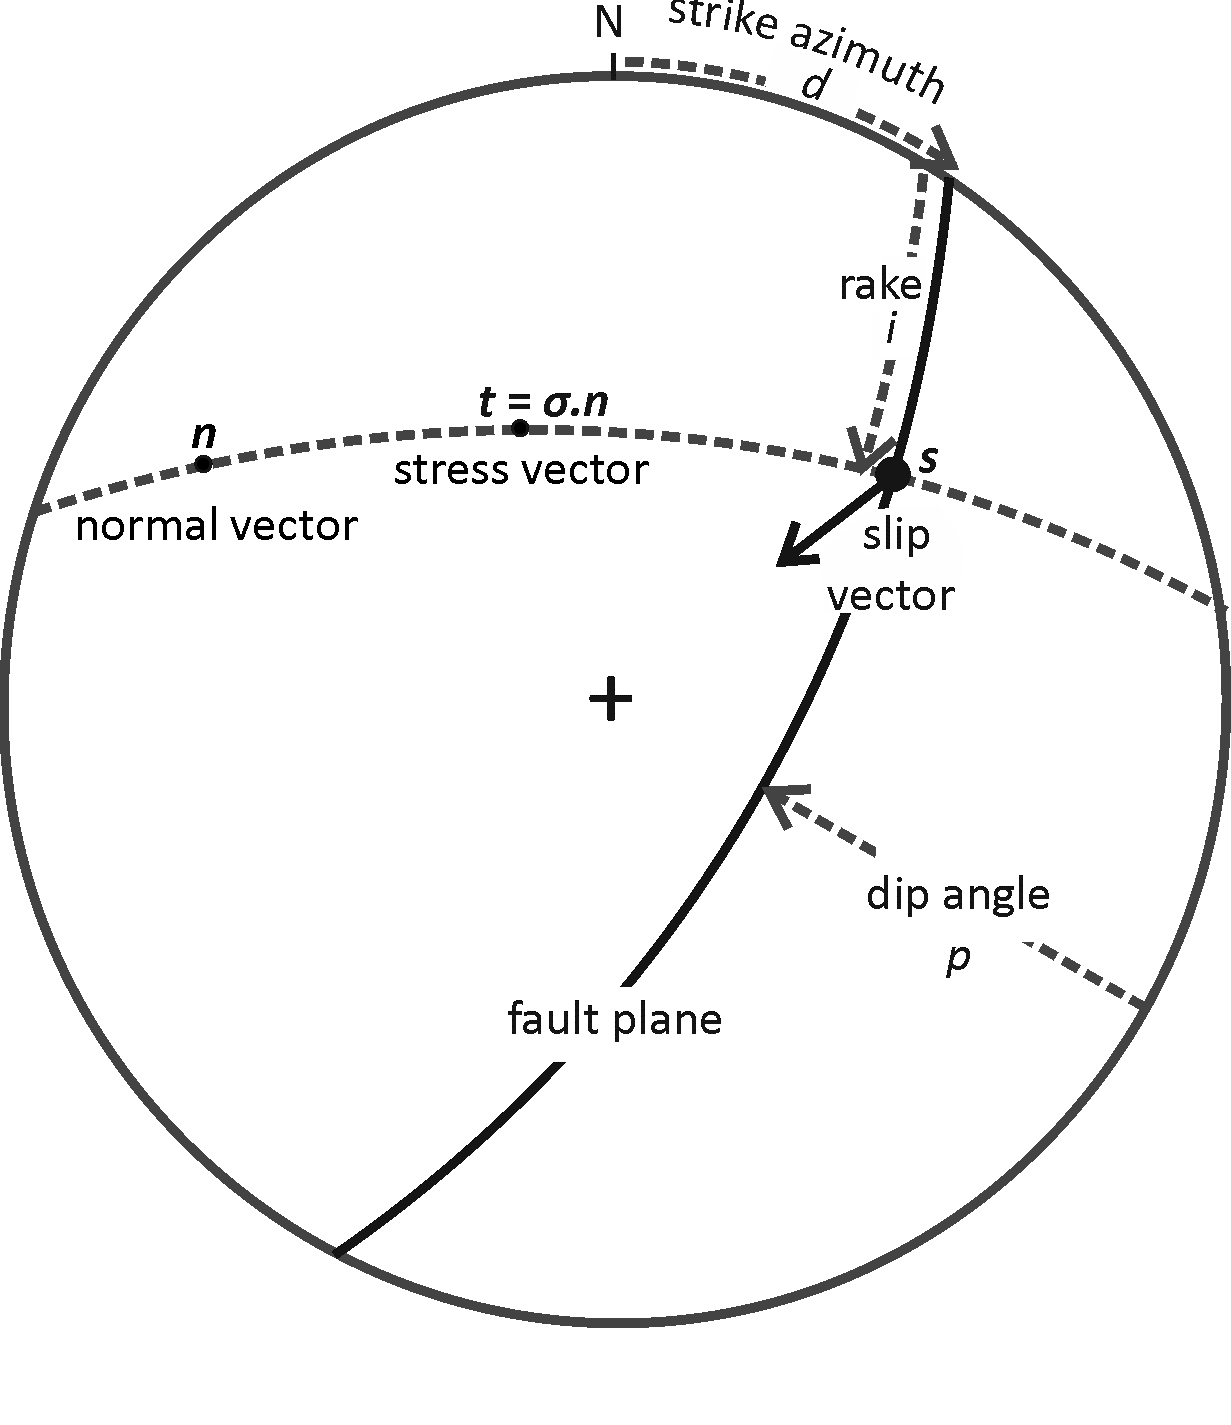
\includegraphics[scale=0.2]{Fig1b}
\caption{Lower hemisphere equal-area projection showing input parameters, $d$, $p$, and $i$, and the stress vectors.}
\label{fig1}
\end{figure}

The normal vector $\bm{n}$ and the slip vector $\bm{s}$ can be expressed in their component form as:
\begin{equation} \label{1}
\begin{split}
n_{x} &= sin(p).cos(d), \\
n_{y} &= -sin(p).sin(d), \\
\text{and}\ n_{z} &= cos(p).    
\end{split}
\end{equation}
\begin{equation} \label{2}
\begin{split}
s_{x} &= cos(i).sin(d) - sin(i).cos(p).cos(d), \\
s_{y} &= cos(i).cos(d) - sin(i).cos(p).sin(d),\\
\text{and}\ s_{z} &= sin(i).sin(p).
\end{split}
\end{equation}

\section{Representation of the Reduced Stress Tensor}
In continuum mechanics, the Cauchy stress tensor, a 3 x 3 symmetric matrix containing six independent parameters, describes the stress acting at a point. We can further reduce this tensor to only four independent variables (Angelier 1994), by eliminating the depth of burial and pore pressure, since it is impossible to estimate them from fault-slip observations (Angelier, 1994). We describe this reduced stress tensor ($\bm{\sigma}$) using three Euler angles ($\alpha$, $\beta$, $\gamma$) (Celerier, 1988; Celerier et al., 2012) and a stress ellipsoid ratio ($\phi$) (Angelier, 1975, 1994). 

\begin{figure}[h]
\centering
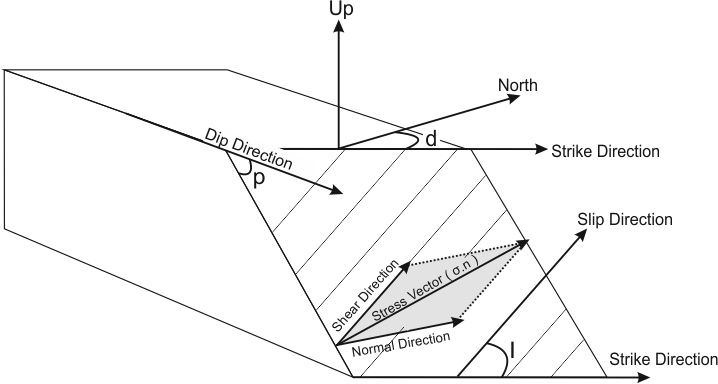
\includegraphics[scale=0.7]{Fig1a}
\caption{Block diagram of a fault surface, showing the normal and shear stress vector components, and the input parameters $d$, $p$, and $i$.}
\label{fig2}
\end{figure}

A symmetric Cauchy stress tensor is given as$-$
\[ 
\begin{bmatrix}
\sigma_{xx} & \sigma_{xy} & \sigma_{xz}\\
\sigma_{xy} & \sigma_{yy} & \sigma_{yz}\\
\sigma_{xz} & \sigma_{yz} & \sigma_{zz}
\end{bmatrix}.
\]
Here, the components along the main diagonal are the eigenvectors of the matrix, which are mutually perpendicular, and the corresponding eigenvalues are called principal stresses. The principal stresses are hereafter referred to as $\sigma_{1}, \sigma_{2}$ and $\sigma_{3}$ in the decreasing order of their magnitudes. The rest of the non diagonal components are called the shear stresses. The shear stresses will vanish in a principal stress frame of reference. Therefore, if we rotate this stress tensor into a principal stress frame, we get the principal stress tensor $ ( \bm{\sigma_{p}} ) - $

\begin{equation}
\label{3}
\bm{\sigma_{p}} =  
\begin{bmatrix}
\sigma_{1} & 0 & 0\\
0 & \sigma_{2} & 0\\
0 & 0 & \sigma_{3}
\end{bmatrix}.
\end{equation}
It is important to note that we cannot completely determine all the values of these principal stresses from fault-slip observations. This is because it is impossible to determine the pore fluid pressure and the depth of burial, unless additional information about friction is given, and because the slip directions are virtually insensitive to these parameters. But we can determine the relative magnitudes of the three principal stresses, and the orientation of these stresses. This parameter $\phi$, called the stress ellipsoid ratio, gives us the shape of the stress ellipsoid (An ellipsoid with the three axes as the principal stress magnitudes).

If we add an isotropic stress tensor $-\sigma_{3}\bm{I}$ (where $\bm{I}$ is the identity matrix) to Eq. \ref{3}, and then multiply the equation with $\frac{1}{\sigma_{1} - \sigma_{3}}$, then we get a reduced stress tensor$(\bm{\sigma_{0}})$ in the principal stress reference frame, given by: 

\begin{equation} \label{4}
\bm{\sigma_{0}} =  
\begin{bmatrix}
1 & 0 & 0\\
0 & \phi & 0\\
0 & 0 & 0
\end{bmatrix},
\end{equation}
and
\begin{equation}
\label{5}
\phi = \frac{ \sigma_{2} - \sigma_{3} }{ \sigma_{1} - \sigma_{3} }.
\end{equation}
  
This tensor can then be rotated to align along the geographic coordinate system, in which the fault geometry is measured. This rotation is described by the Euler angles $\alpha, \beta$ and $\gamma$ (Celerier 1988, Yamaji 2000).

The composite rotation matrix $\bm{R}$ can be written as:
\small
\noindent
\begin{equation} \label{6}
\bm{R} =
\left[
\begin{smallmatrix}
sin(\alpha)sin(\beta) & cos(\alpha)cos(\gamma)-sin(\alpha)cos(\beta)sin(\gamma) & -cos(\alpha)sin(\gamma)-sin(\alpha)cos(\beta)cos(\gamma)\\
-cos(\alpha)sin(\beta) & sin(\alpha)cos(\gamma)+cos(\alpha)cos(\beta)sin(\gamma) & -sin(\alpha)sin(\gamma)+cos(\alpha)cos(\beta)cos(\gamma)\\
cos(\beta) & sin(\beta)sin(\gamma) & sin(\beta)cos(\gamma)
\end{smallmatrix} \right].
\end{equation}

\normalsize
Restricting the maximum principal stress axis to the upper half sphere, we can obtain the ranges of values of the Euler angles as follows (Celerier 1988, 2012) $-$
\begin{equation}
\label{7}
0 \le \alpha < 2\pi; \hspace{3mm} 0 \le \beta \le \frac{\pi}{2}; \hspace{3mm} 0 \le \gamma < 2\pi. \hspace{3mm}
\end{equation} 
Also, from equation \ref{5}, we can deduce that that the range of values of $\phi$ is $-$
\begin{equation}
\label{8}
0 \le \phi \le 1.
\end{equation}
The reduced stress tensor after rotation ($\bm{\sigma}$) can be expressed in terms of ($\bm{\sigma_{0}}$) and the rotation matrix ($\bm{R}$) as-
\begin{equation} \label{9}
\bm{\sigma} = \bm{R}.\bm{\sigma_{0}}.\bm{R^T}.
\end{equation}
Thus, we have a total of four independent variables: the three Euler angles $(\alpha, \beta, \gamma)$ and the stress ellipsoid ratio $(\phi)$ as our output parameters which completely describe the stress tensor  ($\bm{\sigma}$), to be estimated using inversion technique. 

\section{Mechanism of Fault-Slip}
Mohr Coulomb criteria , and adequately explains failure along intact rocks. But it is often seen that the rock masses have a preferred weakness plane, along which they tend to slip. Furthermore, a majority of faults slip along pre-existing fault planes. These pre-existing faults along with faults in anisotropic materials are referred to as reactivated faults. The mechanism of reactivated faults was given by Wallace (1951) and Bott(1959).

Wallace (1951) suggested that the slip in faults occur along the direction and orientation of maximum shear stress. Bott (1959) derived the equations for the same by considering the stress vector acting on different fault planes with variable orientations. This Wallace-Bott hypothesis is also able to explain oblique slip faulting, and hence can be used for non Andersonian stress states as well.

The traction vector ($\bm{T}$) on a fault plane with normal ($\bm{n}$) in terms of the Cauchy stress tensor ($\bm{\sigma}$) is given as (Fig. \ref{fig2}) - 
\begin{equation}
\label{10}
\bm{T} = \bm{\sigma}.\bm{n}.
\end{equation}
The normal and tangential components of this vector (Fig. \ref{fig2}) are the normal and shear traction vectors ($\bm{\sigma_{n}}$ and $\bm{\sigma_{s}}$), given by $-$
\begin{align}
\label{11}
\bm{\sigma_{n}} &= (\bm{n} . \bm{T}) \bm{n} = (\bm{n} . (\bm{\sigma}.\bm{n}))\bm{n},\\
\label{eq:15}
\bm{\sigma_{s}} &= \bm{T} - \bm{\sigma_{n}} = \bm{\sigma}.\bm{n} - (\bm{n} . (\bm{\sigma}.\bm{n}))\bm{n}.
\end{align}
The Wallace-Bott Hypothesis says that this shear stress direction is coincident with the direction of slip, $\bm{s}$, defined in Section \ref{sec:2.1}. Therefore, in terms of $\bm{s}$, the shear stress vector is $-$
\begin{equation}
\label{13}
\bm{\sigma_{s}} = (\bm{s} . \bm{T})\bm{s} = (\bm{s} . (\bm{\sigma}.\bm{n}))\bm{s}.
\end{equation}

\section{The Mean Misfit Function}
The objective function to be minimized for the stress tensor is the sum of misfits between the observed slip direction and the shear component of stress vector (Yamaji 2007). The misfit function is a measure of how well an individual model set satisfies the given set of observations. The misfit angle, $M$, between the two unit vectors ($\bm{\sigma_{s}}/|\bm{\sigma_{s}}|$ and $\bm{s}$) is defined as:

\begin{equation} \label{14}
M = \left|tan^{-1} \left(\frac{|  (\bm{\sigma_{s}}/|\bm{\sigma_{s}}|) \times \bm{s}|}{ (\bm{\sigma_{s}}/|\bm{\sigma_{s}}|) \cdot \bm{s}}\right)\right|.
\end{equation}  

Angelier (1975) suggested the following misfit function for minimization-

\begin{equation} \label{15}
G = sin\left(\frac{M}{2}\right),
\end{equation} 
where $0 \le M < 2\pi$. This function minimizes the angular misfit between the two vectors, the observed slip direction and the predicted direction of maximum shear stress.

Another minimization function, which minimizes the misfit between the magnitudes of shear components, is (Angelier et al., 1982):

\begin{equation} \label{16}
H = \left| \bm{s} . (\bm{\sigma}.\bm{n}) - \sqrt{( (\bm{\sigma}.\bm{n})^2 - (\bm{n} . (\bm{\sigma}.\bm{n}))^2 )} \right|.
\end{equation}

We define a misfit function, $F$, that accounts for both, the angular misfit $G$ and the magnitude misfit of the shear component $H$, as:

\begin{equation} \label{17}
F = \lambda G + (1-\lambda) H,
\end{equation}
where $\lambda$ is the weighting parameter in the range $0 \le \lambda \le 1$. A similar function is described by Delvaux and Sperner (2003).The mean misfit function $\bar{F}$, is average of the $F$ for all the faults in a given population, and this function is minimized for determination of the reduced stress tensor.

\chapter{GA Methodology}
\lhead{\emph{3. GA Methodology}}
\thispagestyle{empty}
\onehalfspacing
The GA is an adaptive search technique derived from the Darwinian theory of natural selection: the individuals having greater fitness will have better chances of survival in a population of organisms. We use this theory as the basis for stress inversion and formulate a minimization problem. Since there are only four unknowns in the reduced stress tensor but a much larger number of fault-slip observations, the inverse problem is over-constrained and a best-fit tensor needs to be determined.

In this optimization problem, the domain of the output parameters is the search space. The initial population, a fixed number of individuals, is sampled randomly from the search space. Analogous to the genetic evolution, the initial population of stress tensors undergoes reproduction, through the natural processes of selection, crossover and mutation, iteratively. We explain each of these processes in the context of stress inversion.

\section{Initialization and Encoding}
We use stochastic sampling to produce an initial population of models, each model set $(\alpha, \beta, \gamma, \phi)$ representing a possible solution to the inverse problem, i.e., a reduced stress tensor. The model parameters are encoded in a binary string, and each model set is referred as a chromosome. The length of the chromosome is dependent upon the number of parameters and the desired resolvability of each parameter.

The four model parameters that describe the reduced stress tensor are each encoded as a 6-bit binary string, making the chromosome 24 bits long (Fig. 2). The mapping of these parameters in real space depends on their ranges defined in the preceding section.

\begin{figure}[h]
\centering
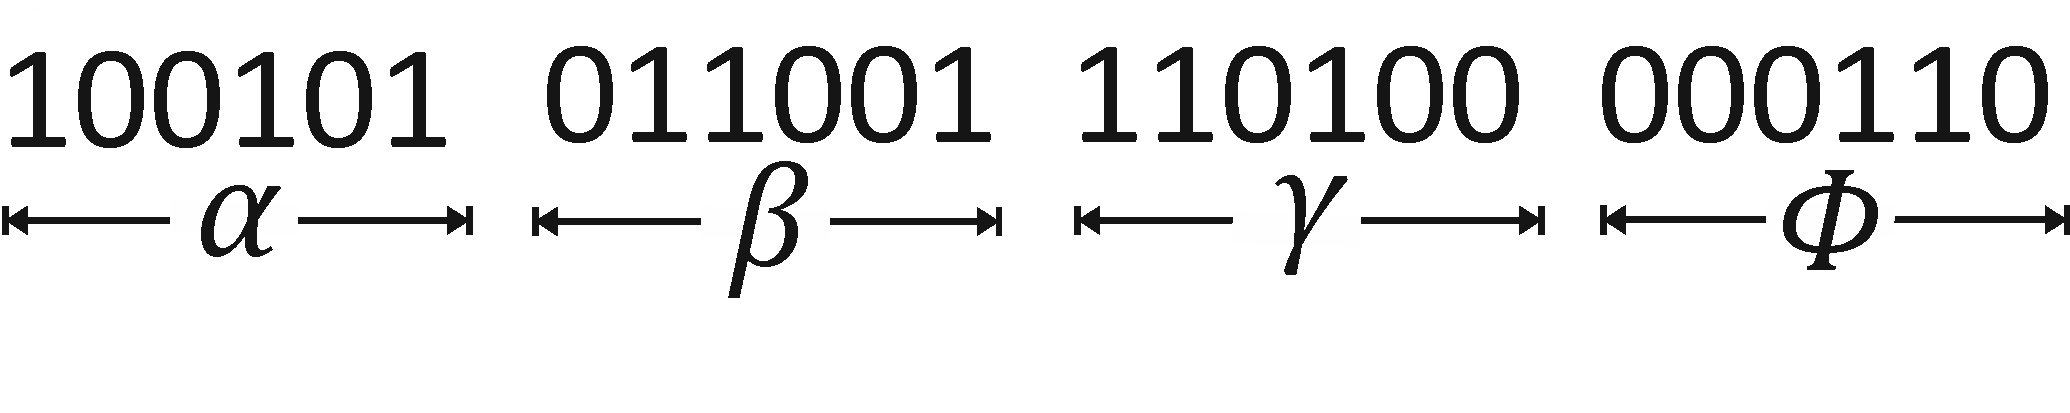
\includegraphics[scale=0.15]{Fig3}
\caption{A chromosome containing 24 binary bits, 6 in each of the four parameters, the three Euler angles ($\alpha, \beta, \gamma$) and the stress-ellipsoid ratio ($\phi$).}
\label{fig3}
\end{figure}

\section{Selection}
The initial population is generated randomly, and each model set is ranked according to the mean misfit function, $\bar{F}$. The next step is to select the best-fit candidates for reproduction. Among a wide range of options that exists for selection, we use the most popular method, the tournament selection. Several tournaments are played between randomly chosen individuals and the winners are selected for mating. Although the misfit criteria decides the winner, the selection of the individuals is essentially stochastic, which prevents the possibility of extinction of a potentially good fit offspring.

\section{Crossover}
Crossover involves exchange of bits between two selected individuals, called `parent models`, to produce two new individuals, called `offspring models`. This is analogous to the exchange of genetic material during reproduction, where the child inherits certain characteristics from both the parents. 
A fixed percentage of previously selected chromosomes, 80\% as a rule of thumb, undergo crossover in the manner described below: (Fig. 4A-C):
\renewcommand{\theenumi}{\roman{enumi}}
\begin{enumerate}
    \item Two crossover sites, e.g., 8th and 15th in Fig. 3A, are randomly selected in the parent chromosomes containing four variables of 6 binary bits each, i.e., 24 bits in total.
    \item The bits lying between the two sites are exchanged between the two parents to produce two offspring (Fig. 4B).
\end{enumerate}

\section{Mutation}
Mutation prevents a rapid convergence of the algorithm to a local optimum. It occurs by flipping a randomly chosen bit in either of the offspring. For example, mutation occurs by flipping the 14th bit from 0 to 1 in the second offspring in Fig. 4B-C. It is carried out with a probability that is low enough to allow the convergence of the solution and high enough so that the solution is not trapped in a local optimum. The probability of mutation is generally taken as 1/(number of bits). Mutation also allows for the possibility of having a better-fit individual, whose characteristics cannot be derived from either parents.

\begin{figure}[h]
\centering
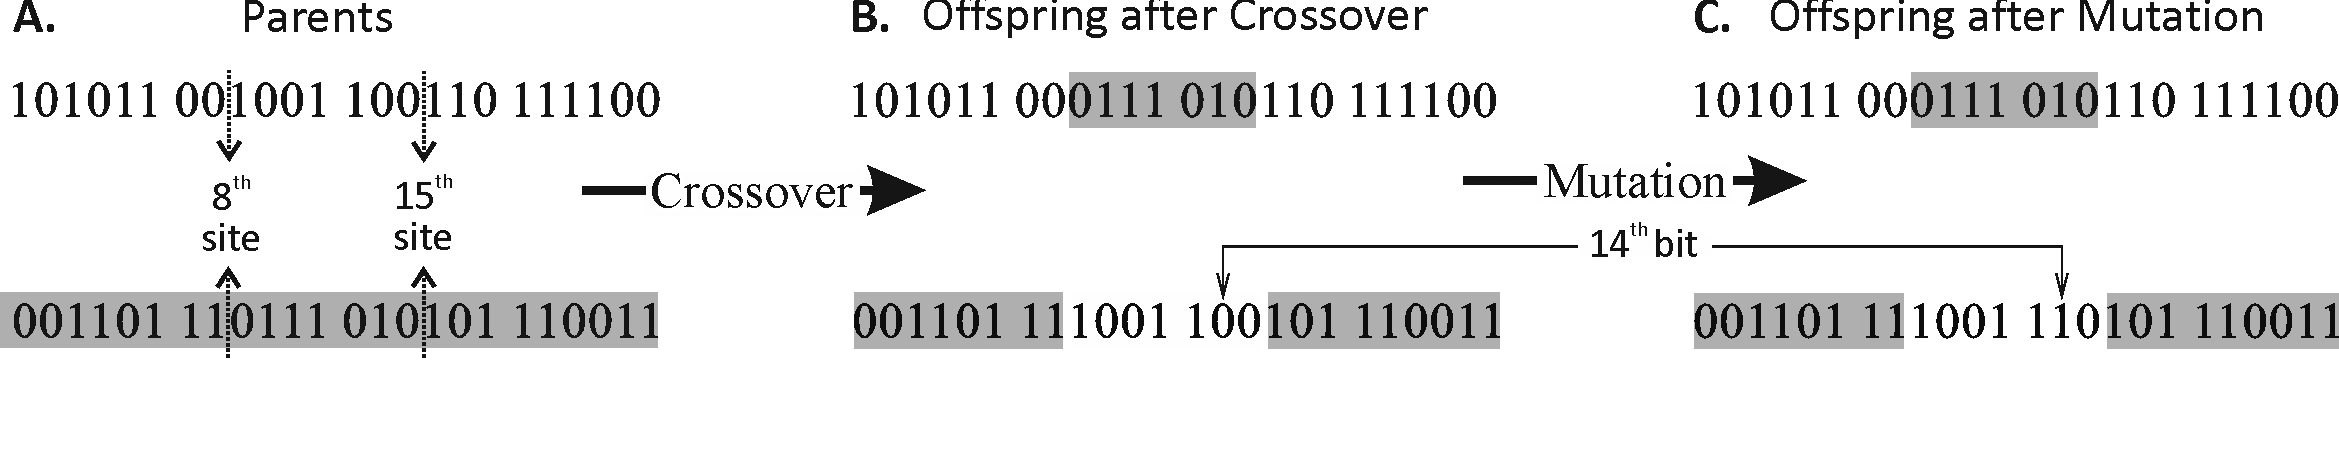
\includegraphics[scale=0.23]{Fig4}
\caption{\textbf{A}: A pair of parents each having 24 binary bits. \textbf{B}: A pair of offspring produced after exchange of bits at two random crossover sites, 8th and 15th, in this case. \textbf{C}: Mutation in the second offspring by flipping of the 14th bit from 0 to 1.}
\label{fig4}
\end{figure}

\section{Termination Criteria}
The pool of the candidates at this stage consist of a fixed percentage of original members and newly created offspring models. The pool is then treated as the next generation that undergoes selection, crossover and mutation again. This process repeats until the mean misfit function stabilizes (Fig. \ref{fig5}).

\begin{figure}[H]
\centering
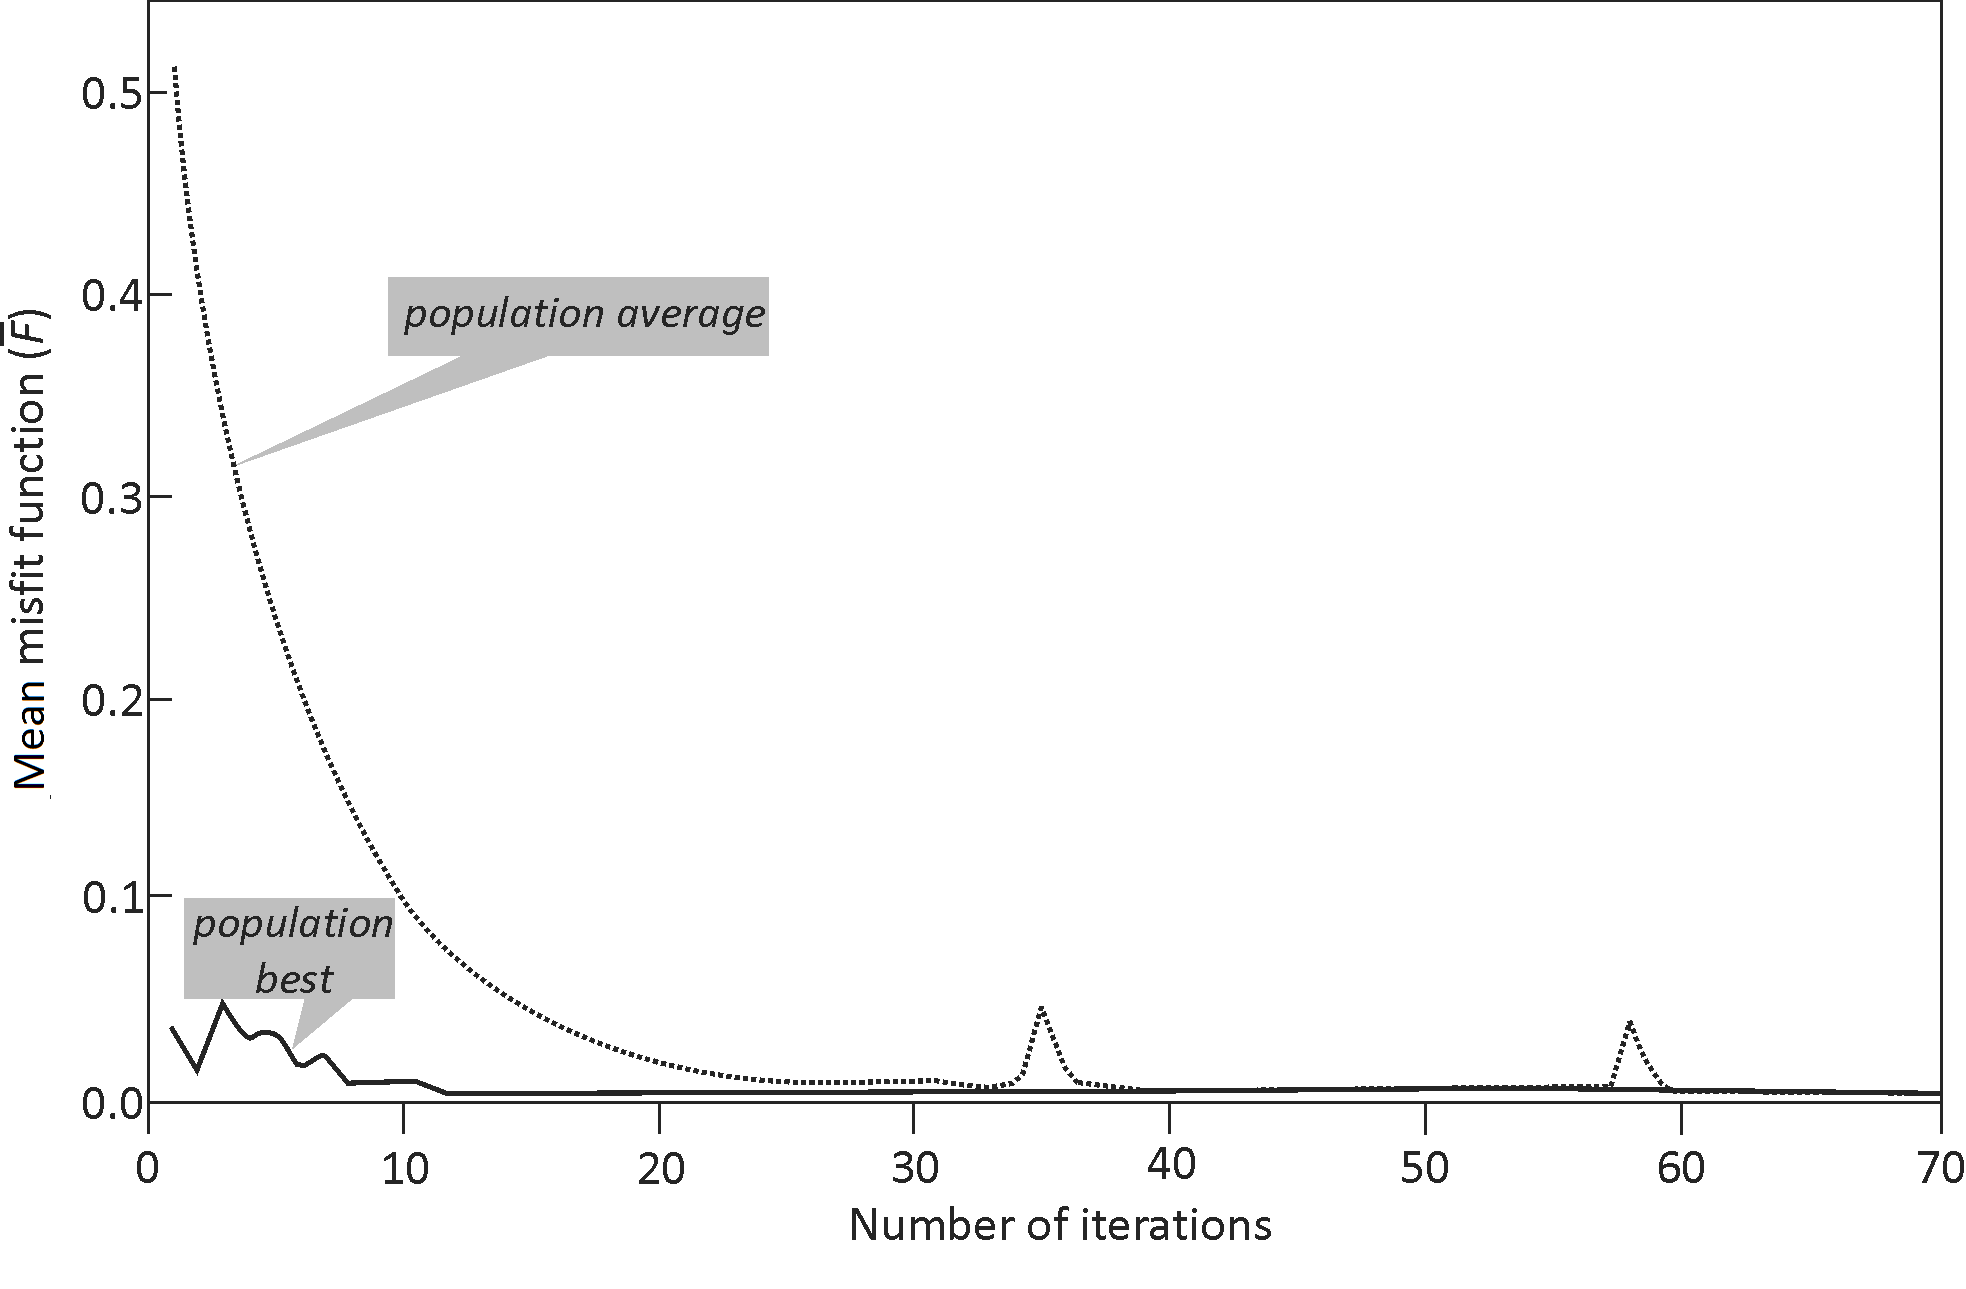
\includegraphics[scale=0.26]{Fig5}
\caption{Convergence curve of the mean misfit function $\bar{F}$ with iterations. Small peaks are caused by chromosomes with mutations.}
\label{fig5}
\end{figure}

\chapter{Validation of the GA Inversion}
\lhead{\emph{4. Validation of the GA Inversion}}
\thispagestyle{empty}
\onehalfspacing
We demonstrate the success of the GA on synthetically simulated ideal and noisy fault-slip observations, and an example of published fault-slip observations from Tymbaki, Greece (Angelier, 1979).

\section{Synthetic Fault-Slip Observations}
Given a reduced stress tensor, we compute the direction and sense of shear stress/slip on a fault plane. We have randomly sampled the strike and dip values for simulations. These values follow a uniform probability density function. Only those striated fault planes are used that obey the Byerlee’s law (1978), i.e., the ratio of the shear to the normal stress $\ge$ 0.85. Using known values of the reduced stress tensors, synthetic fault-slip observations are simulated for extensional, compressional, strike-slip and oblique tectonic settings (Fig. 6A-D). The first three tectonic settings are defined by vertically directed $\sigma_{1}$, $\sigma_{2}$ and $\sigma_{3}$ respectively, whereas none of the principal stresses are vertical in the oblique tectonic setting. Each set of synthetically simulated fault-slip observations is analysed by the GA and the results are compared with true values in the known stress tensors. In all the four tectonic settings, the results given by the GA are consistent with the true values in respective reduced stress tensors (Table 1).

We have also used the synthetic fault-slip observations for comparison of the GA with other common methods, the 4-D exploration (Angelier, 1984) and the direct inversion (Angelier, 1990). These methods also produce acceptable results in situations where one of the principal stresses is vertical (Table 1). However, in the oblique tectonic settings, where none of principal stresses are vertical, these methods may give results that deviate significantly from the true values (Table 1). This may be attributed to the possibility that the inversion becomes highly nonlinear when the axes are inclined and the direct methods get trapped in a locally optimum solution. Similarly, in the existing implementations of the 4-D exploration, a starting point of the algorithm is predefined using the inversion results from the direct inversion, hence the results tend to be similar. A detailed analysis of all the methods are required to further comment upon this deviation, which is beyond the scope of this study.

\section{Noisy Fault-Slip Observations}
Data sets obtained from the fault-slip observations in field are commonly noisy. To test the effect of noise on the GA, we added eight percent random noise, following the uniform distribution, to the each of the synthetic observations strike, dip and rake in oblique tectonic setting (Fig. 6D) and obtained the noisy data set (Fig. 6E). For noisy data, the GA produces results that have deviation commensurate with noise added to data (Table 1). This choice of noise percentage is arbitrary and as the noise percentage increases, so will the deviation from the true value.

\section{Natural Fault-Slip Observations}
We have tested the validity of the GA on many natural fault-slip observations. Here, we present a typical test on a natural example of fault-slip observations from Tymbaki, Greece (Angelier, 1979, 1990). This example has been commonly used for testing the validity of different methods (Michael, 1984; Hardcastle and Hills, 1991; Yin and Ranalli, 1995). The results from GA compare well with those given by the direct inversion and the 4-D exploration (Fig 6F, Table 2). It is noteworthy that the principal stress orientations are close to Andersonian orientation in this example.

\pagebreak
%\begin{landscape}
\begin{table}[H]
  \footnotesize
  \centering
  \renewcommand{\arraystretch}{1.5}
  \begin{tabular}{@{}ccccccccc@{}}
    \toprule
    \multicolumn{4}{c}{True values (Given stress tensor)} & Method & Ratio & \multicolumn{3}{c}{Principal stress orientation} \\
    
    \midrule
    
    $\phi$ & $\sigma_1$ & $\sigma_2$ & $\sigma_3$ & & $\phi$ & $\sigma_1$ & $\sigma_2$ & $\sigma_3$ \\
    
    \cmidrule(lr){1-4} \cmidrule(lr){6-9}
  
    0.20 & 000/90 & 090/00 & 000/00 & 4D & 0.21 & 011/89 & 269/00 & 179/01 \\
    
    \multicolumn{4}{c}{Extensional Setting (Fig. 6A)} & DI & 0.20 & 152/90 & 270/00 & 000/00 \\
    
    \multicolumn{4}{c}{ } & GA & 0.21 & 000/90 & 090/00 & 000/00 \\
    \midrule
    
    0.90 & 180/00 & 090/00 & 000/90 & 4D & 1.00 & 224/00 & 314/00 & 077/90 \\
    
    \multicolumn{4}{c}{ Compressional Setting (Fig. 6B)} & DI & 0.90 & 357/00 & 087/00 & 226/90 \\
     
    \multicolumn{4}{c}{ } & GA & 0.89 & 180/00 & 090/00 & 000/90 \\
    \midrule
    
    0.40 & 180/00 & 000/90 & 270/00 & 4D & 0.40 & 179/03 & 356/87 & 089/00 \\
    
    \multicolumn{4}{c}{ Strike-slip Setting (Fig. 6C)} & DI & 0.43 & 180/01 & 338/89 & 090/00 \\
     
    \multicolumn{4}{c}{ } & GA & 0.41 & 180/00 & 270/89 & 270/01 \\
    \midrule

     0.50 & 134/50 & 334/38 & 236/10 & 4D & 0.61 & 319/66 & 146/24 & 055/03 \\
    
    \multicolumn{4}{c}{ Oblique Setting (Fig. 6D)} & DI & 0.49 & 320/72 & 148/18 & 057/02 \\
     
    \multicolumn{4}{c}{ } & GA & 0.44 & 137/52 & 332/37 & 237/07 \\
    \midrule

     0.50 & 134/50 & 334/38 & 236/10 & 4D & 0.76 & 318/78 & 163/22 & 072/05 \\
    
    \multicolumn{4}{c}{ Noisy Data (Fig. 6E)} & DI & 0.65 & 332/78 & 165/11 & 075/03 \\
     
    \multicolumn{4}{c}{ } & GA & 0.33 & 150/55 & 342/34 & 249/06 \\
    \midrule
    \multicolumn{9}{l}{\textit{Note}:4D- 4D exploration, DI- Direct Inversion, GA- Genetic Algorithm.}
    \bottomrule
  \end{tabular}
  \caption{Test of GA on synthetic examples and comparison with other methods.}\label{table:1}
\end{table}

\begin{table}[H]
  \footnotesize
  \centering
  %\renewcommand{\arraystretch}{1.5}
  \begin{tabular}{@{}ccccc@{}}
    \toprule
    Method & Ratio & \multicolumn{3}{c}{Principal stress orientations}\\
    \cmidrule(lr){2-5} \\
     &  $\phi$ & $\sigma_1$ & $\sigma_2$ & $\sigma_3$ \\
    \midrule
    
    4D & 0.07 & 275/82 & 057/06 & 147/05 \\
    DI & 0.05 & 186/85 & 065/03 & 335/04 \\
    GA & 0.06 & 100/79 & 044/06 & 315/09 \\
    
    \midrule
    \multicolumn{5}{l}{\textit{Note}: Abbreviations same as Table 1.}
    \bottomrule
  \end{tabular}
  \caption{Application of GA on a natural example and its comparison with other methods.}\label{table:2}
\end{table}

\begin{figure}[H]
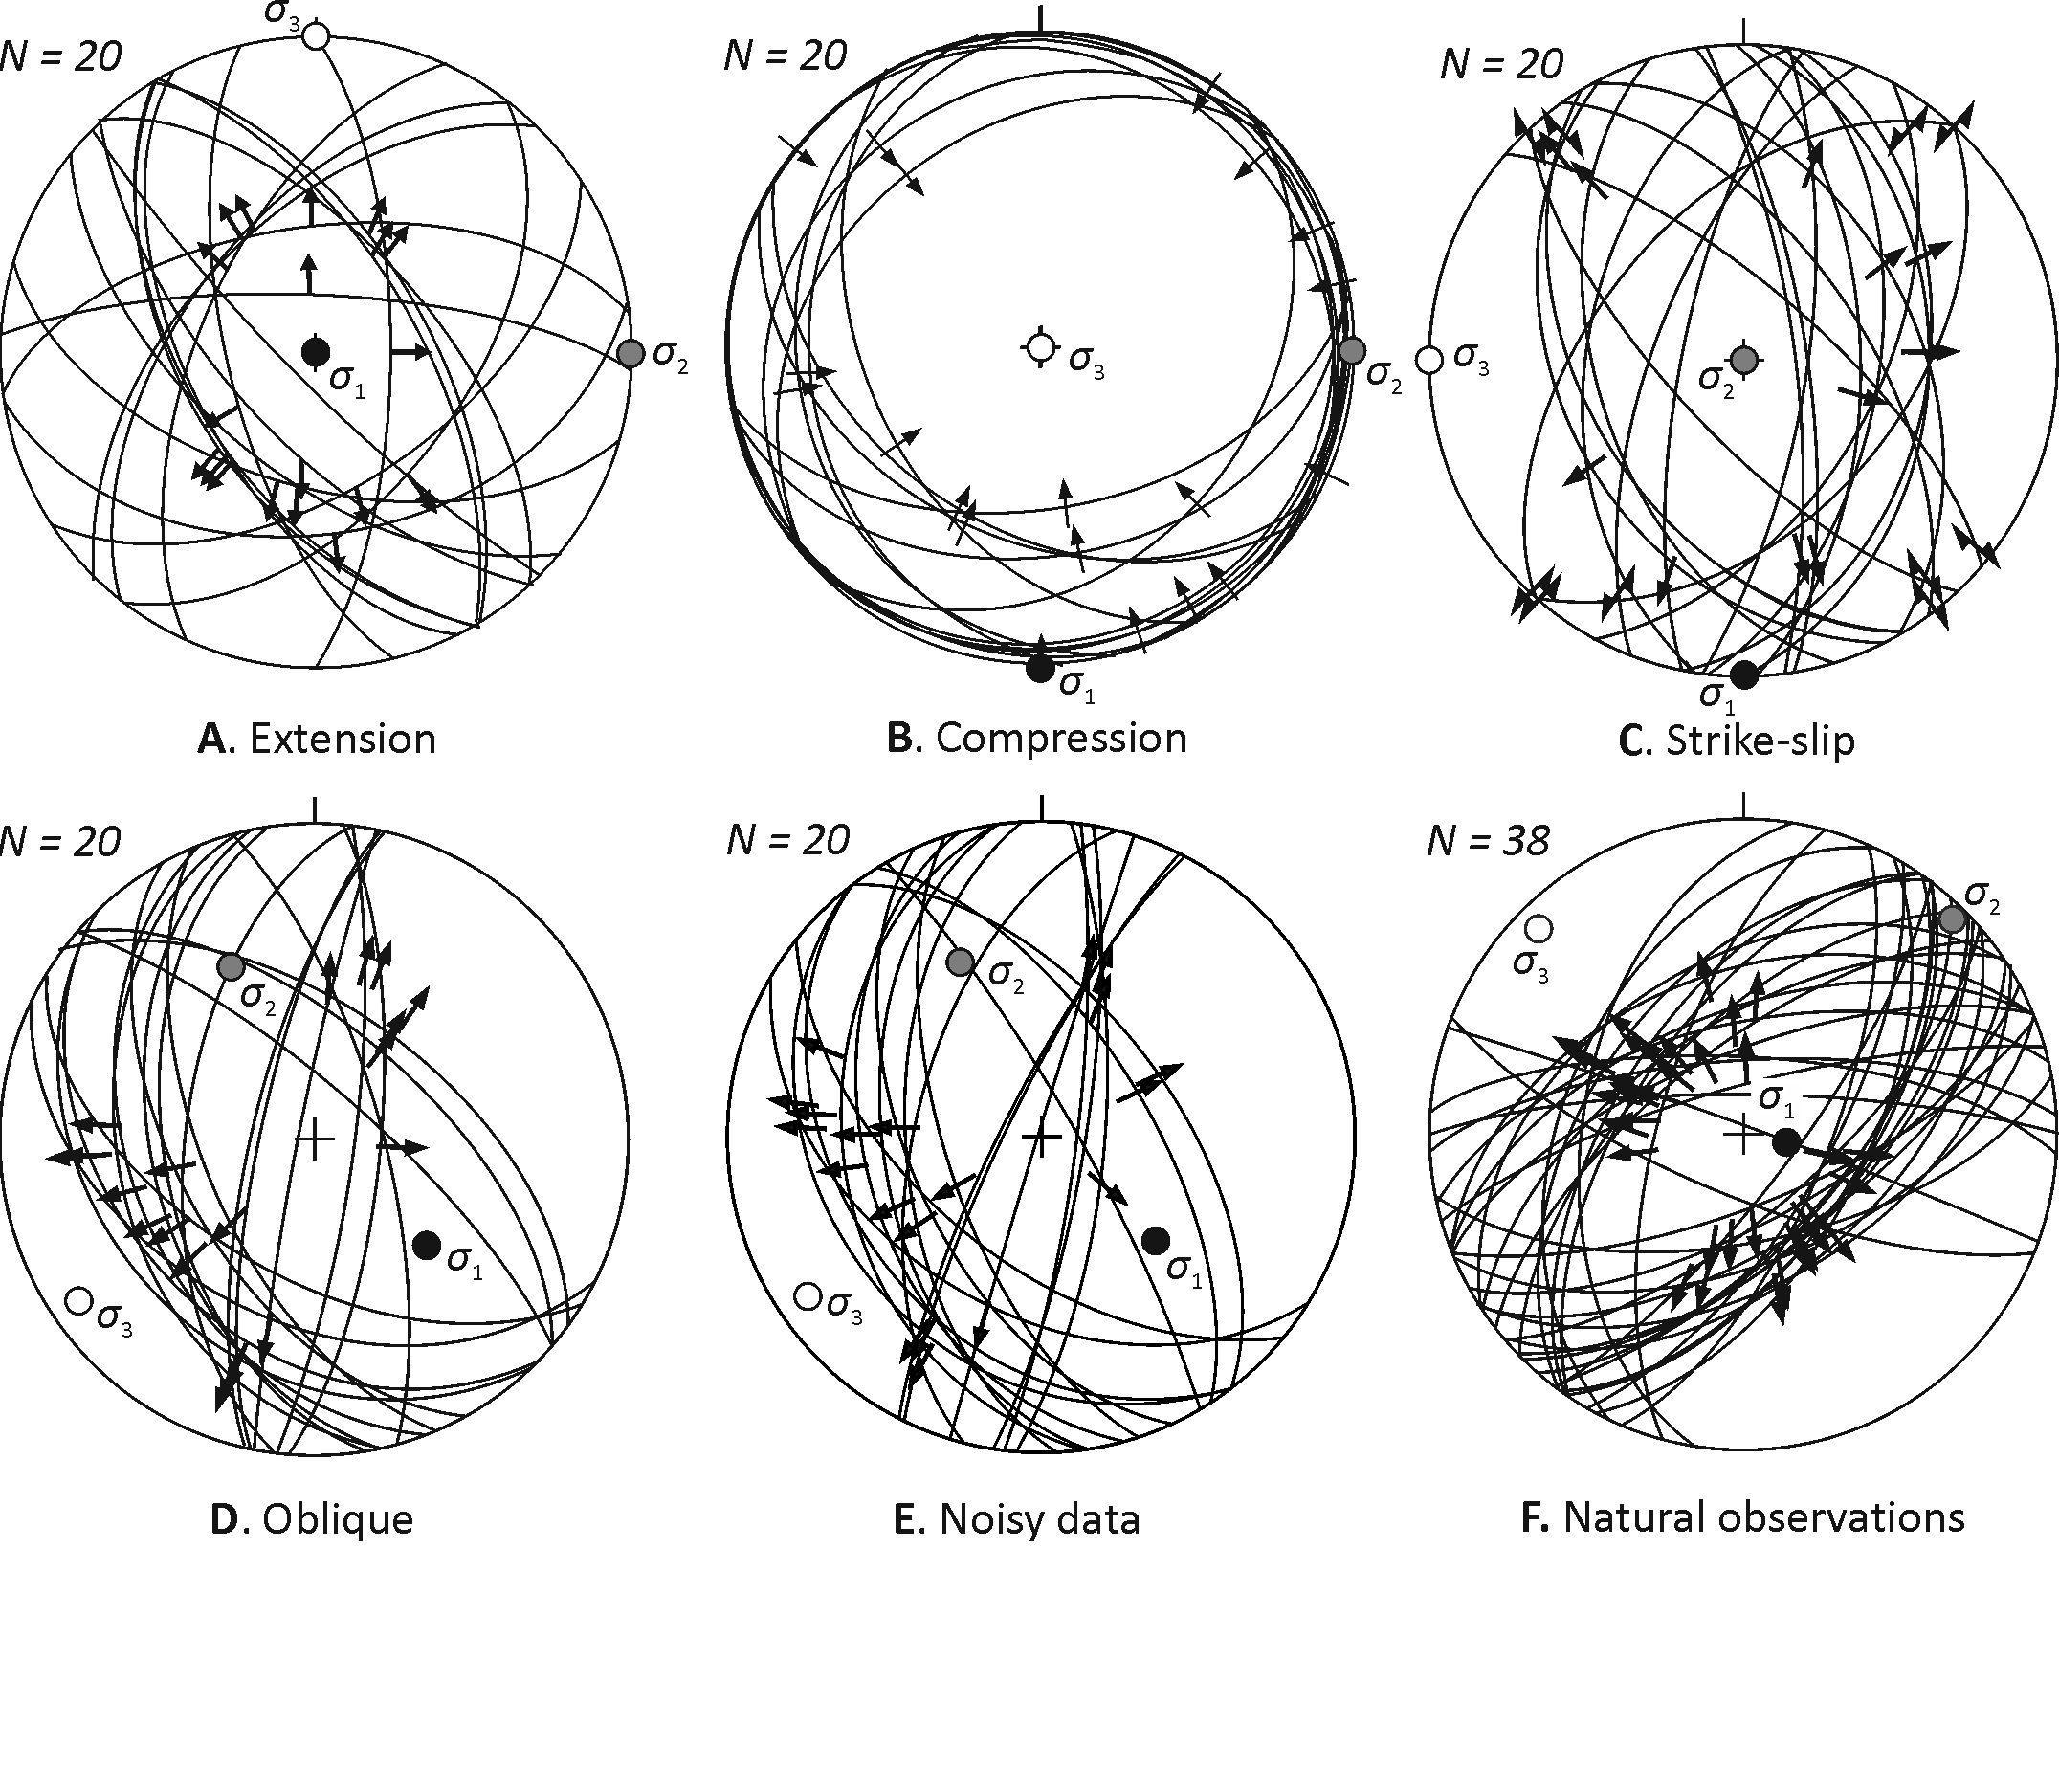
\includegraphics[scale=0.24]{Fig6}
\caption{Validation of the GA. \textbf{A-E}: Synthetic fault-slip observations in four different tectonic settings. \textbf{A}: Extensional, \textbf{B}: Compressional, \textbf{C}: Strike-slip, \textbf{D}: Oblique tectonic setting. \textbf{E}: Noisy data set. \textbf{F}: Natural fault-slip observations (Angelier, 1979).}
\label{fig6}
\end{figure}

\cleardoublepage
\begingroup
  \makeatletter
  \let\ps@plain\ps@empty
  \part{Separation of Polyphase Fault-slip data using the Genetic Algorithm}
\endgroup

\chapter{Introduction}
\lhead{\emph{5. Introduction}}
\thispagestyle{empty}
\onehalfspacing
Typical inversion of fault-slip observations involves minimizing the sum of angular misfits between the observed and the theoretical slip direction to yield a best fit stress tensor. A number of methods have been proposed for this task (Carey and Brunier, 1974; Angelier, 1979; Angelier et al., 1982; Michael, 1984; Xu, 2004). These methods work well when it is known that all the observations belong to a single stress regime. Quite often, we have multiple phases of faulting occurring in nature, caused by successive events, where each phase is characterized by its own stress tensor. In the region of polyphase faulting, where more than one stress tensor is at play, these inversion techniques will yield meaningless results. It is one of the most challenging tasks for a geologist to separate the different phases of faulting before inverting the observations to find the stress tensor. 

In order to separate the polyphase fault-slip observations into single phase subsets, a variety of methods have been proposed. These methods can be broadly grouped into search methods (Hardcastle and Hills, 1991; Shan et al., 2007) and clustering methods (Nemcok and Lisle, 1995; Yamaji, 2000; Shan et al., 2003). Search methods use exhaustive grid search to group the observations into subsets based on a deviation threshold (Hardcastle and Hills, 1991). This threshold is defined by the user, hence the division of the observations is subject to bias. Furthermore, these methods have difficulty in separating stress tensors with similar orientations. Clustering methods try to group similar faults-slip observations together based on similarity of fault-slip data and/or stress vectors. The Multiple Inverse Method (Yamaji, 2000) inverts every possible quadruplet in the data set, and then groups the data with similar tensors. The Cluster Analysis method (Nemcok and Lisle, 1995) follows a hierarchical clustering approach which uses a similarity coefficient based on a range of trial stress tensors to produce a dendogram. The major limitation with existing clustering methods is that they require visual inference from the user in order to decipher the phases in an unknown fault-slip data set.

Fry (1999) showed that stresses are linearly separable in a six dimensional hyperplane. A number of methods have built upon this formulation of the stress inversion problem to separate polyphase fault-slip data sets (Shan et al., 2003; Shan and Fry, 2005; Hansen et al., 2015). Shan and Fry (2006) pointed out that these methods may only give correct results if the stress associated with the smallest eigenvector is unique. Furthermore, methods using iterative procedures (Shan et al. 2003) have difficulty in overcoming locally optimized division. Shan et al. (2007) have given a method to overcome this limitation, using a grid search approach. This approach is very time consuming and the approach taken for obtaining the optimum number of subsets is an empirical approach and lacks a theoretical basis. For a detailed review of these existing methods and their shortcomings, the reader is directed to (Nemcok et al., 1999; Shan et al., 2003; Leisa and Lisle 2004).

To sum up, two important problems in the existing methods are: (i) finding out the number of phases in the given data, and (ii) difficulty in reaching the globally optimized solution. Some methods circumvent the problem of optimal division of subsets using fuzzy clustering (e.g. Shan et al., 2004), while other methods qualitatively estimate the best division (e.g. Nemcok and Lisle, 1995; Yamaji, 2000).
We design a Genetic Algorithm based Polyphase Separation (GAPS) technique that separates polyphase fault-slip observations from a set of stress tensors, based on the misfit criteria. The GAPS is a robust heuristic search technique that separates the fault-slip data without any assumption about the number of stress states. It reaches the globally optimum solution by using stochastic search and selection rules.


\chapter{Methodology}
\lhead{\emph{6. Methodology}}
\thispagestyle{empty}
\onehalfspacing
We use the genetic algorithm in order to classify the fault-slip observations into its respective stress regimes. Genetic algorithm is a heuristic search technique adapted from the Darwinian theory of natural selection, and is quite often used in nonlinear optimization problems (Holland, 1975; Goldberg, 1989; Sen and Stoffa, 1995). A few methods use k-means cluster analysis in combination with the genetic algorithm (Liu et al., 2011) for classification, but to the best of our knowledge, the genetic algorithm itself has never been used to separate and invert the data simultaneously. 

If we referring back to Section 2.2 and 2.3, Chapter 2, we can recall that the input parameters for the inversion are normal and slip vectors, $\bm{n}$ and $\bm{s}$ and the output parameters are the three Euler angles ($\alpha$, $\beta$, $\gamma$) and the stress ellipsoid ratio ($\phi$). We will collectively refer to this output parameter set as $O$ ($ = [\alpha, \beta, \gamma, \phi]^T$).

\section{Observations Containing $M$ Phases of Stresses}
Let the $N$ number of input parameters belong to $M$ phases of multiple stress tensors. Our task is to classify each of these $N$ input parameters into one of the $M$ stress tensors, using the misfit criteria. We begin with an initial set of possible solutions (initialization), calculate their misfit, and perform the genetic operations elitism, selection, encoding, crossover and mutation iteratively. Each of these steps is described in brief below.

\subsection{Initialization}
Initialization involves randomly generating a large number of output parameters, $O$, in their domain, defined in Section 2.3, Chapter 2. This is called the initial population, and its size is called the population size. In the GAPS, the initial population, $\bm{P}$, is a column vector of length $L$, the population size.
\begin{equation} \label{18}
\bm{P} =
\begin{bmatrix}
\bm{P_1} \\
\vdots \\
\bm{P_i} \\
\vdots \\
\bm{P_L}
\end{bmatrix}.
\end{equation}

Each member of this initial population is a row vector with $M$ rows, corresponding to the number of phases in the data. The elements of this row vector are randomly initialized output parameters $O$. Thus, the $i^{th}$ member of the initial population $\bm{P_i}$, is:
\begin{equation} \label{19}
\bm{P_i} = 
\begin{bmatrix}
O_1 & \dots & O_M
\end{bmatrix}.
\end{equation}

We compute the stress tensor corresponding to each output parameter set $O$.

\subsection{Misfit Calculation}
The next step is to calculate the misfit of each member of the initial population. The $i^{th}$ row of the initial population has $M$ stress tensors. We use Eq. (17) to obtain the misfit of each input parameter set with respect to each of the $M$ stress tensors. We define an $N \times M$ matrix called the Data Misfit Matrix ($\bm{DMM}$), for one member of the initial population, as follows:
\begin{equation} \label{20}
\bm{DMM} = 
\begin{bmatrix}
F_{11} & \dots & F_{1M}\\
\vdots & \ddots & \vdots\\
F_{N1} & \dots & F_{NM}
\end{bmatrix}.
\end{equation}

Each element of this matrix is the function $F$ defined for a particular observation and a particular stress phase. In order to classify each observation into one of the $M$ stress tensors, we define an Index Matrix, $\bm{IM}$, as follows:
\begin{equation} \label{21}
IM_{ij} = \left\{
\begin{matrix}
 1 & if DMM_{ij} = \displaystyle \min_{j \in M} DMM_{ij},\\
 0 & otherwise.
\end{matrix} \right
\end{equation}

Note that each row of the index matrix will have only one non-zero element, since each observation can belong to only one stress phase. The number of non-zero elements in $j^{th}$ column of the $\bm{IM}$ is the number of observations belonging to the $j^{th}$ stress tensor. This is the initial separation of observations, after the first iteration. Next, we calculate the element-wise product of the matrices $\bm{DMM}$ and $\bm{IM}$ to obtain a matrix $\bm{EP}$:
\begin{equation} \label{22}
EP_{ij} = DMM_{ij} \times IM_{ij}. 
\end{equation}

Now, we take the mean of all the non-zero elements in each column of $\bm{EP}$, and add them to obtain a single value. This is called the composite misfit ($CM$) for one member of the initial population.
\begin{equation} \label{23}
CM = \displaystyle \sum_{i=1}^{M}\left[ \frac{\displaystyle \sum_{j=1}^{N}EP_{ij}}{\displaystyle \sum_{j=1}^{N}IM_{ij}}\right].
\end{equation}

We compute the composite misfit for each member of the initial population. This gives us a vector of length $L$, called the Composite Misfit Vector ($\bm{CMV}$). Next, we sort the $\bm{CMV}$ in increasing order of the composite misfit values. The individual having a lower value is considered a better fit individual and is preferred over the one having a higher value.

\subsection{Elitism}
The top 5\% best fit individuals, having the lowest composite misfit values, are given the privilege of going directly to the next generation. This step, called `elitism`, helps in faster convergence of the solution and also ensures that the best solution is always carried on to the next iteration. The number `5\%` is arbitrary, and it is best decided by forward modelling by using a variety of synthetic data sets to design the algorithm.

\subsection{Selection}
From the remaining 95\%, we select random pair of individuals and compare their fitness. The one with smaller misfit is considered a better fit individual and is chosen to reproduce. This process is called tournament selection. Tournaments are played $0.95*L$ times so that we have 0.95*L winners for reproduction. The set of winners is referred to as the mating pool.

\subsection{Encoding}
The individuals in the mating pool are referred to as parents, and they undergo reproduction via the processes of crossover and mutation, to produce new offspring. These processes of the genetic algorithm operate on binary encoded values of the mating pool. The length of the binary numbers depends on the desired resolvability of the components of O. Assuming each component of O has $b$ binary bits, we divide their ranges (Section 2.3, Chapter 2) into $2^b$ equal parts, and obtain a binary equivalent of the real values. This binary equivalent of the mating pool is also referred to as the mating pool. For our problem, we assume the value of $b = 6$.

\subsection{Crossover and Mutation}
Crossover and mutation alter the bits in the parents to produce new offspring. These operations are analogous to the genetic reproduction in living beings, where the child (offspring) inherits certain characteristics of both the parents.

Crossover operates on two parents, selected randomly from the mating pool, where we interchange the bits between a selected common crossover site on both the parents (Fig. 4A-B). This process allows the algorithm to explore the search space without performing an exhaustive grid search. The probability of occurrence of crossover in the GAPS is 60\%. 

Mutation makes changes to a single parent, by flipping a randomly selected bit from 1 to 0 or 0 to 1 with a very low probability (Fig. 4B-C). This adds randomness to the algorithm, and prevents it from converging too fast. It also results in the solution not getting entrapped in a locally optimum solution, which is prominent if the convergence is too fast. 

This entire process is repeated iteratively, till the population converges and the misfit stabilizes (Fig. 5). In essence, we are attempting to find those tensors which give minimum possible misfit for N number of different data permutations. This ensures that we are selectively minimizing the input vectors, and the algorithm converges to the point where the sum of misfits is minimum for each phase.

\begin{table}[h!]
\centering
\footnotesize
 \renewcommand{\arraystretch}{1.2}
\begin{tabular}{l l}
    \hline
    Symbol & Explanation \\
    \hline
    $DC$ & Direction Cosine \\
    $\bm{n}$ & Normal Vector \\
    $\bm{s}$ & Slip Vector \\
    $\alpha$, $\beta$, $\gamma$ & Euler Angles \\
    $\phi$ & Stress Ellipsoid Ratio \\
    $\bm{\sigma}$ & Stress Tensor \\
    $\bm{\sigma_s}$ & Shear Stress Direction \\
    $M$ & Misfit Angle \\
    $G$ & Angular Misfit Function \\
    $H$ & Magnitude Misfit Function \\
    $F$ & Misfit Function used in this Study\\
    $\bm{P}$ & Initial Population \\
    $L$ & Population Size \\
    $M$ & Number of Phases \\
    $N$ & Number of Observations \\
    $i, j, k$ & Indices of Matrix, Vector \\
    $\bm{DMM}$ & Data Misfit Matrix \\
    $\bm{IM}$ & Index Matrix \\
    $\bm{EP}$ & Element-wise Product of $\bm{DMM}$ and $\bm{IM}$ \\
    $CM$ & Composite Misfit \\
    $\bm{CMV}$ & Composite Misfit Vector \\
    \hline
\end{tabular}
\caption{List of symbols and their meanings.}
\label{table:1}
\end{table}

\section{Determining the Number of Phases}
In the real geological conditions, the number of phases of faulting is usually not known. But for a reasonably realistic condition, this number does not exceed 7 (Shan et al., 2007), and is often around 2-3. In order to determine the number of clusters or phases of faulting events, we run the algorithm successively for 1, 2, 3 phases. Then we compare the mean composite misfit value for each algorithm run. At the optimum number of clusters, the mean composite misfit will have a minimum value.

Another observation made during the test is that when we run the algorithm assuming a larger number of phases than what is present in the data, we often find that one of the phases of separation contains less than four input vectors, giving meaningless inversion results. This can be used as an identifier to determine the number of phases in a much faster way rather than testing it for the different number of phases sequentially. This of course assumes that there are no outliers in the data and we have at least four observations of each phase of stress tensor.


\chapter{Results}
\lhead{\emph{7. Results}}
\thispagestyle{empty}
\onehalfspacing
We simulated homogeneous sets of synthetic data for given stress tensors by generating slip on a series of randomly oriented fault planes. Then, we artificially mixed homogeneous sets to create a polyphase fault-slip data. Three types of tests are carried out, described as follows:

\section{Subsets with Similar Orientations}
We mixed two homogeneous synthetic data sets with same orientations of the principal stress axes, but different stress ellipsoid ratios (Table 4). The results of separation (Fig. 7A) show that GAPS is able to satisfactorily separate the polyphase data set with similar orientation of stresses, and only one fault in each phase is misclassified.

\section{Relatively Uneven Subsets}
In the second test, the polyphase data consists of slip generated on 5 faults from one stress tensor, and slip generated on 15 faults from a different stress tensor. The results, presented in Fig. 7B, show the efficacy of GAPS to separate the data having relatively uneven number of observations points in each phase.  Leisa and Lisle (2004) showed that some methods, such as the Multiple Inverse Method (Yamaji, 2000), fail to separate this type of data set.

\section{Separation of Homogeneous Fault-slip Data}
In the third test, we run the GAPS on a homogeneous data set with two prescribed phases of separation. The results clearly show that one of the phases of separation is minor, and has less than four data points (Fig. 7C). Since our inversion problem consists of four variables to be estimated, the phase with less than four fault slip data obviously gives meaningless inversion results. This phase should be ignored, and we conclude that only one phase is present in the fault-slip data. 

The reason that GAPS gives one phase with less than four data points is entirely related to the composite misfit, that we use for inversion. Since we are minimizing the sum of mean misfit for each phase of faulting, one of the following cases is possible when we overestimate the number of phases in the fault-slip data, which is a single phase in this example:

\renewcommand{\theenumi}{\roman{enumi}}
\begin{enumerate}
    \item The data is separated into the prescribed number of phases, with each phase having more than four data sets. In this case, the inversion of each phase will point towards the same stress tensor, and will tell us exactly how many different stress tensors are present.
    \item The data is separated into the prescribed number of phases, with some of the phases having less than four data sets. In this case, we ignore the phases with less than four data sets, and only consider the inversion results of the significant phases, that have more than four sets.
\end{enumerate}

After numerous trials, we find that the second case is almost always prevalent in the GAPS, and we can determine the number of phases of faulting in a single algorithm run. In order to get more reliable results, and not exclude any of the data, we can then run the algorithm a second time with known number of phases in the data.

\begin{figure}[H]
\begin{subfigure}{\textwidth}
    \centering
    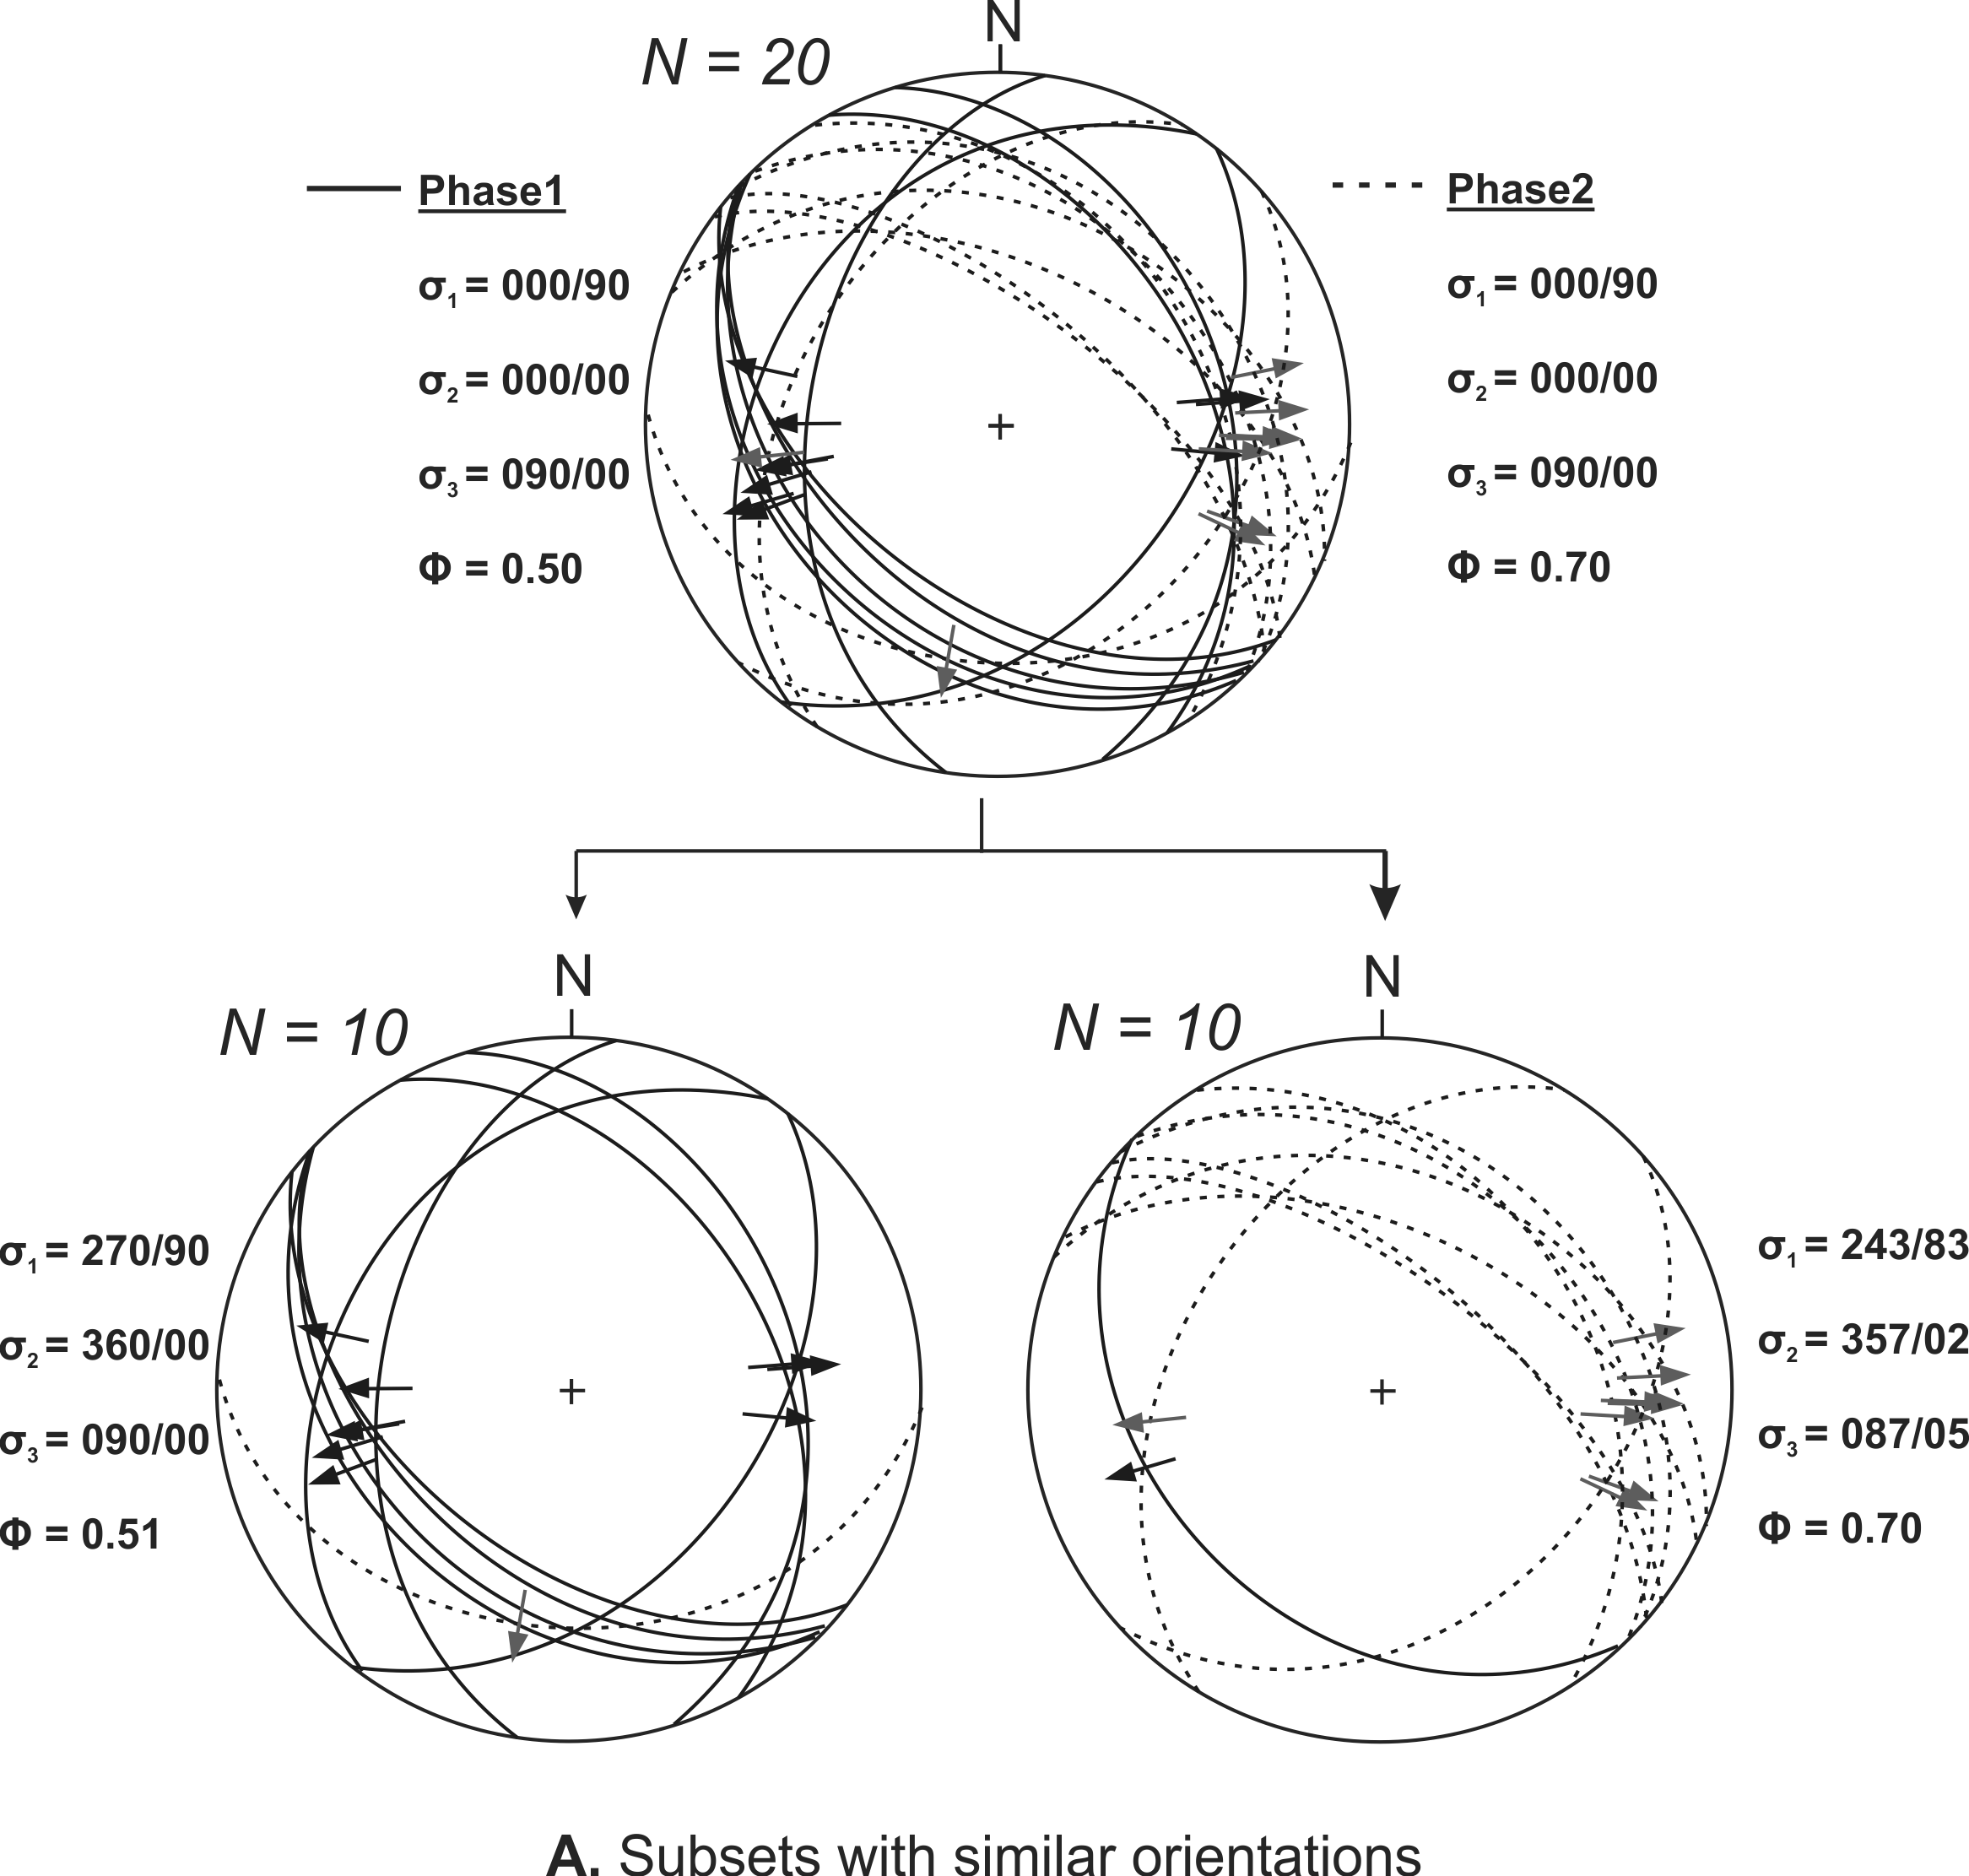
\includegraphics[scale = 0.6]{result2}
\end{subfigure}
\end{figure}
%\pagebreak
\begin{figure}[H]
\ContinuedFloat
\begin{subfigure}{\textwidth}
    \centering
    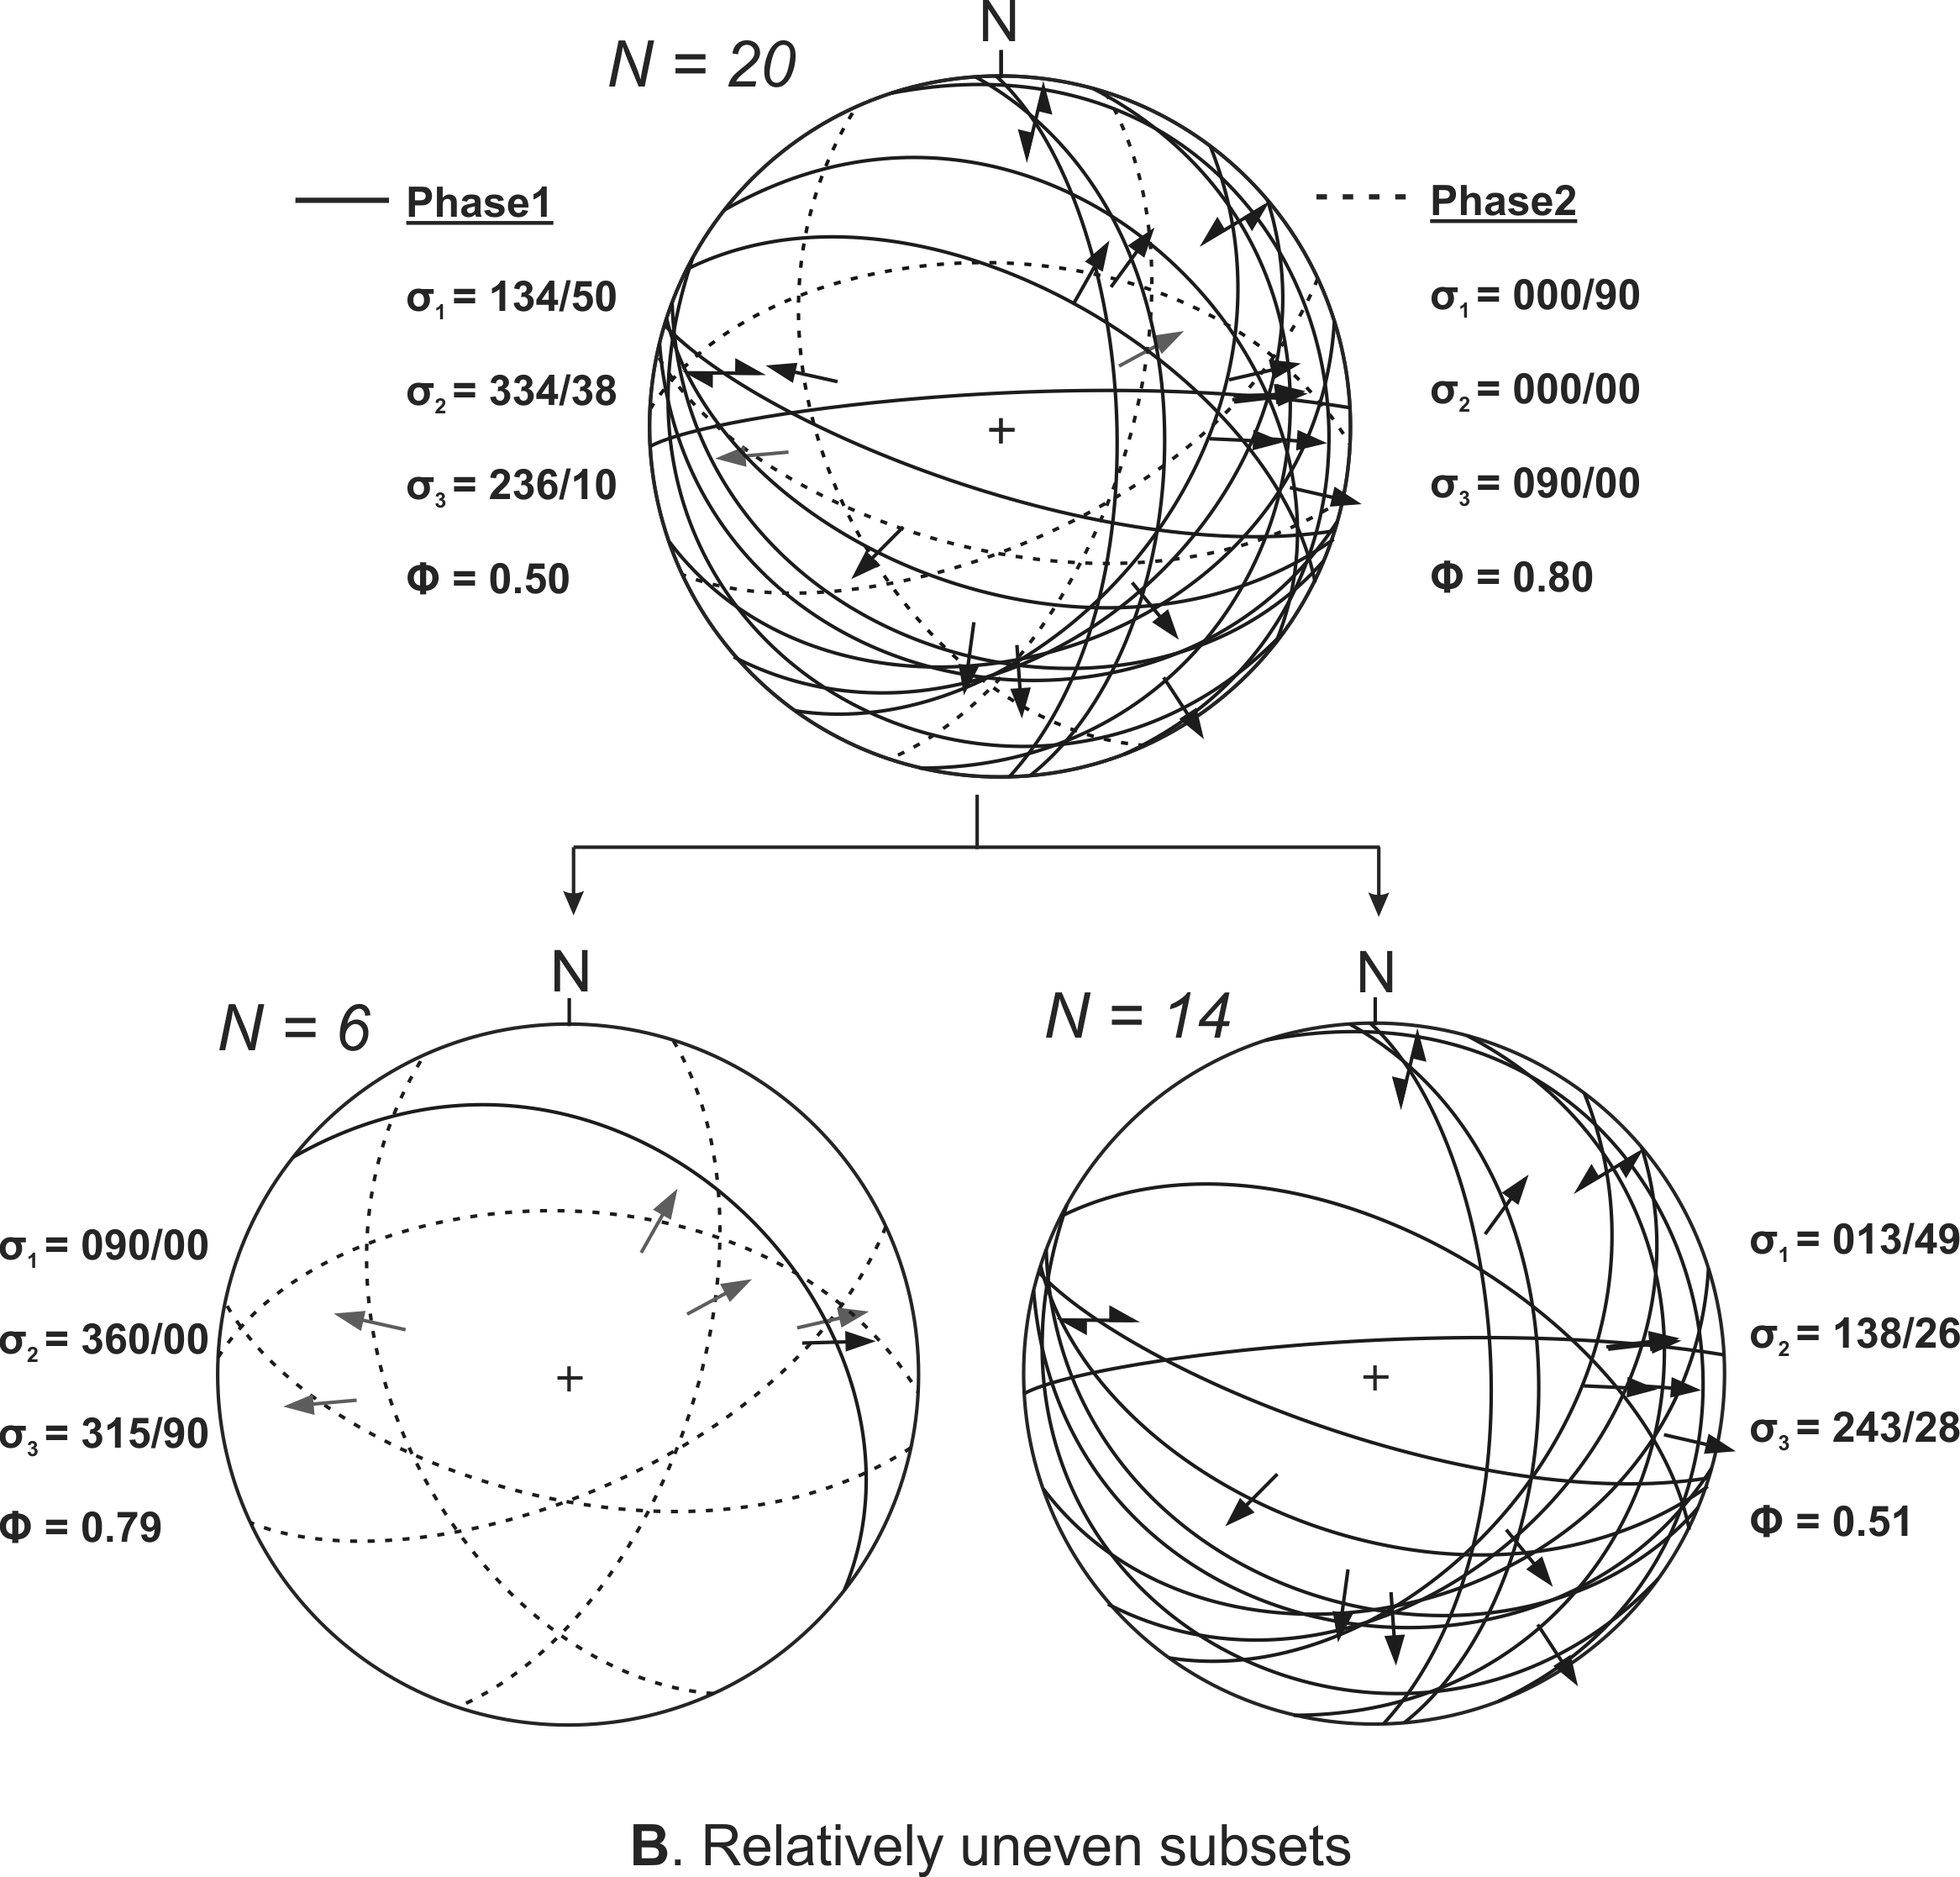
\includegraphics[scale = 0.6]{result2b}
\end{subfigure}
\end{figure}
\begin{figure}[H]
\ContinuedFloat
\begin{subfigure}{\textwidth}
    \centering
    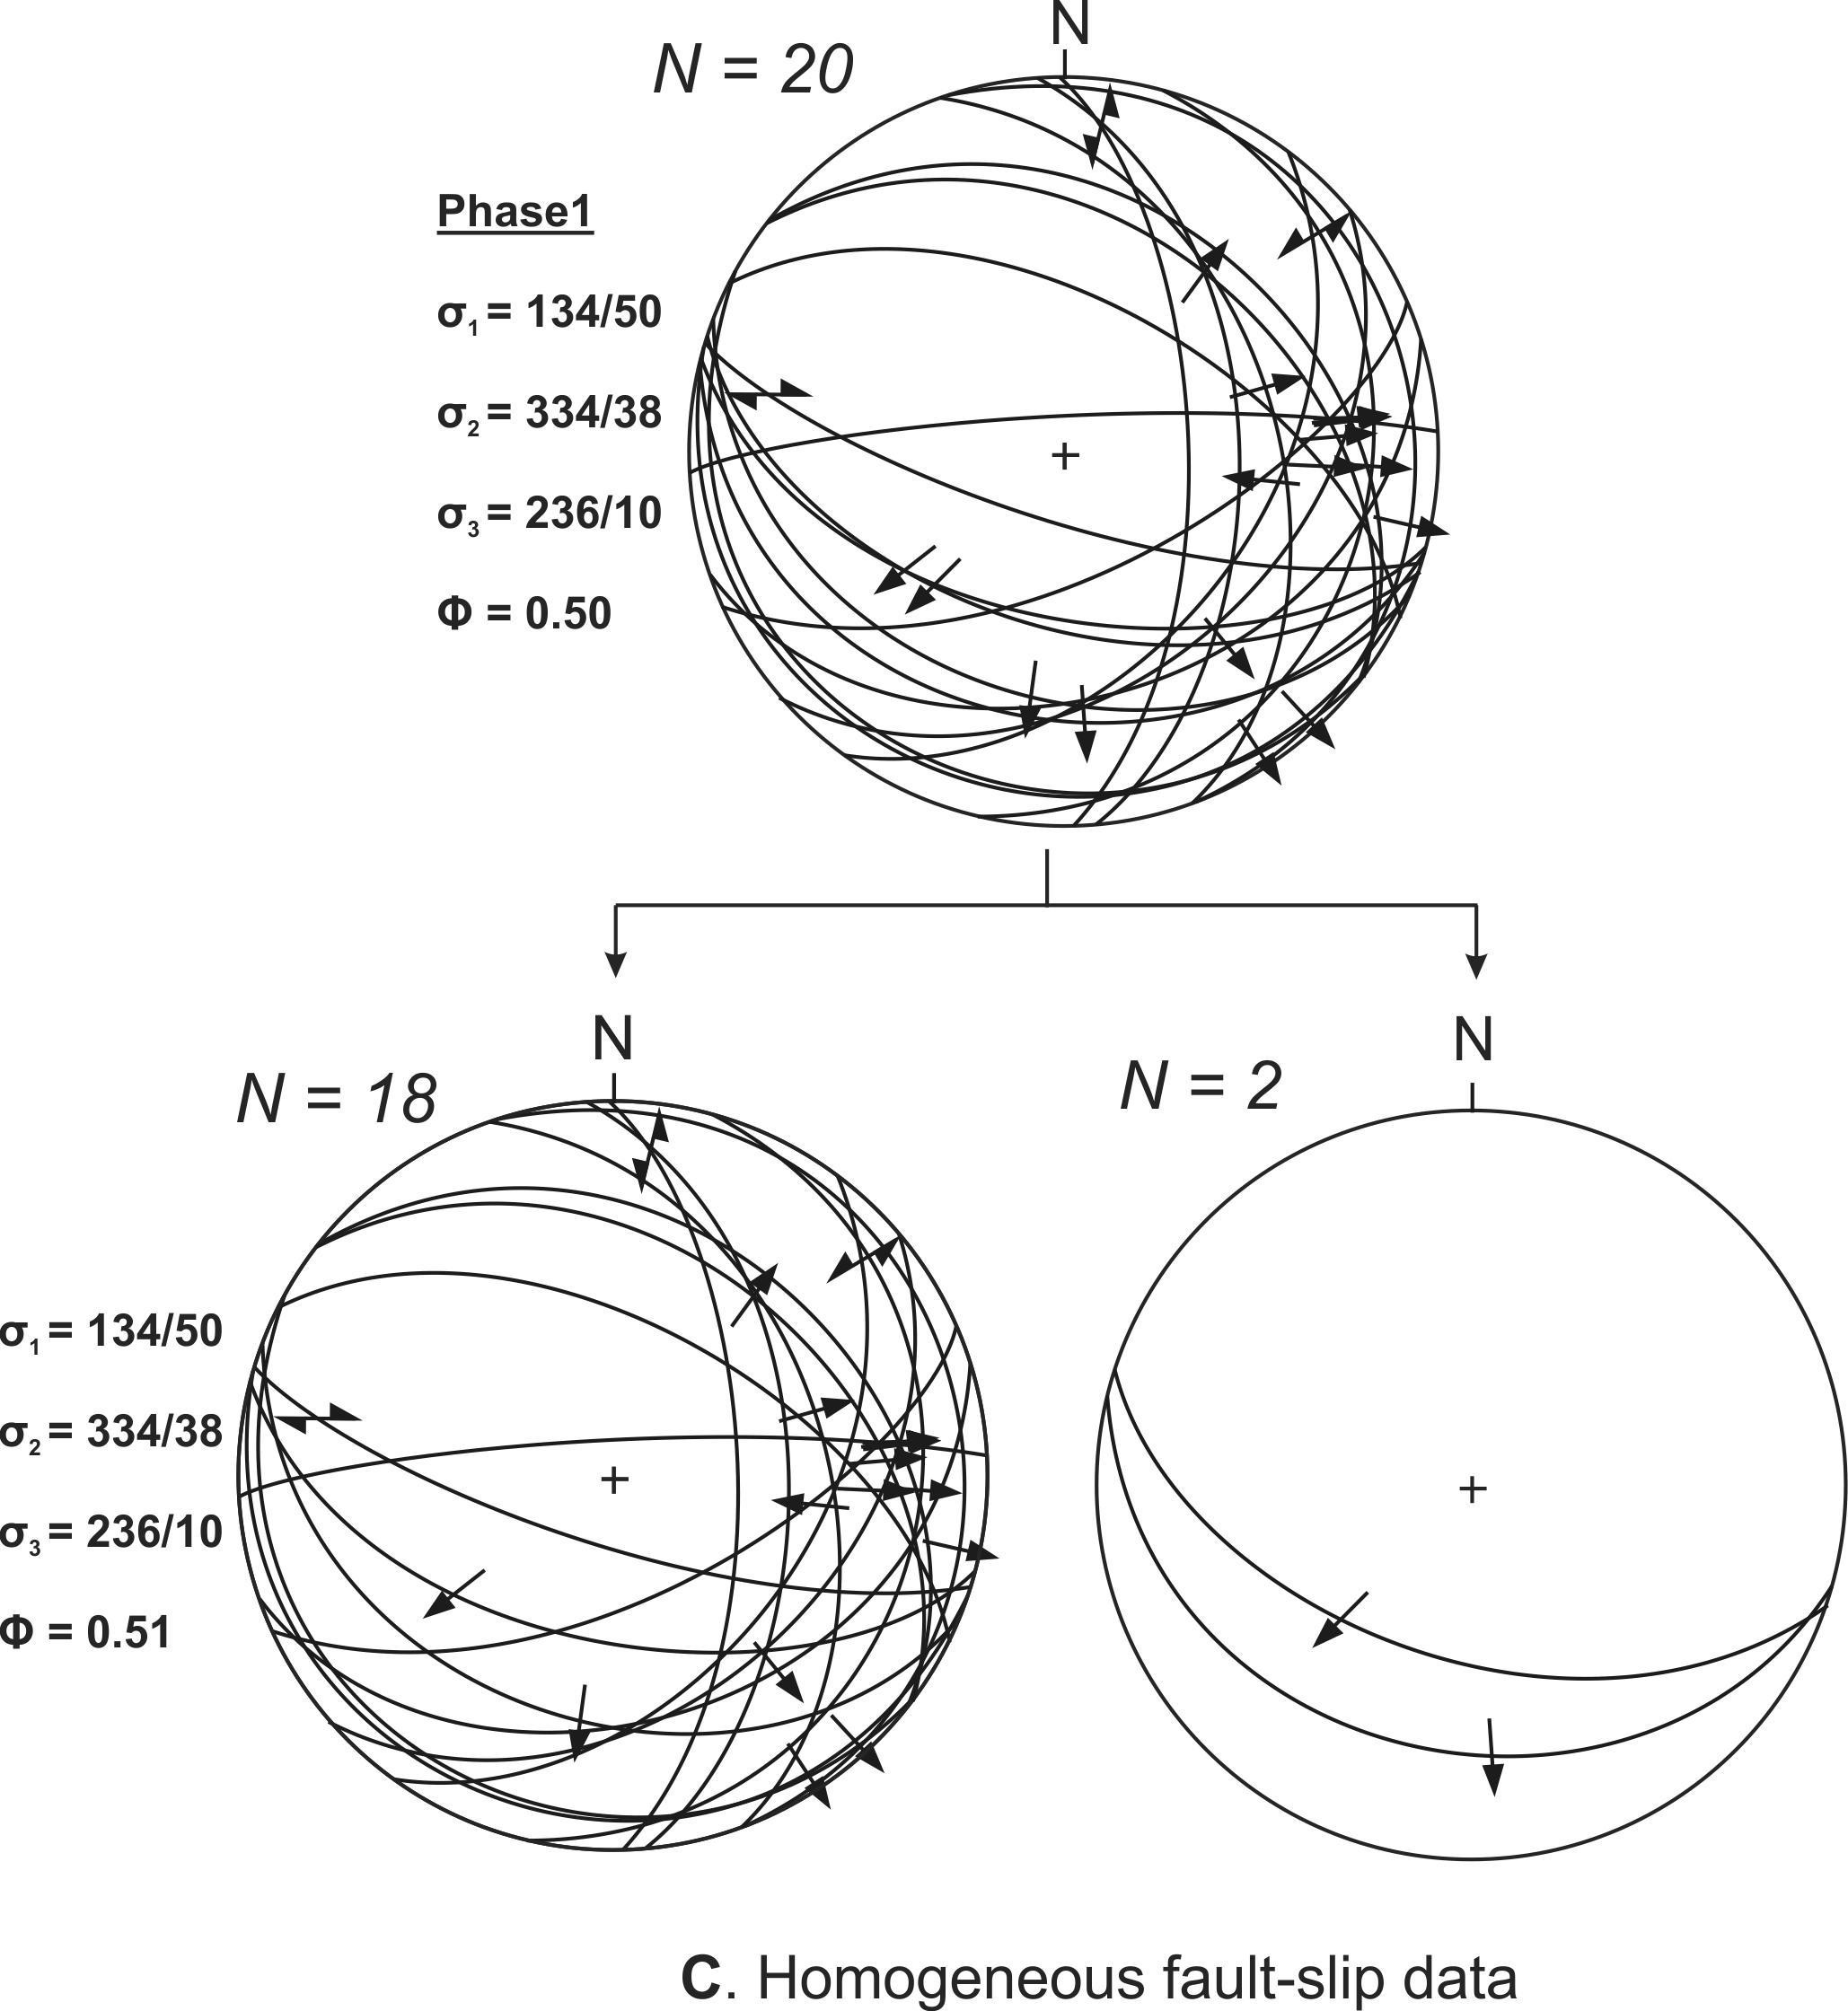
\includegraphics[scale = 0.6]{result2c}
\end{subfigure}
\caption{Separation of polyphase synthetic data sets. The top stereonet shows the synthetic mixed data set, and the bottom stereonets show the separation results.\textbf{A:} Subsets with similar orientation. \textbf{B:} Relatively uneven subsets. \textbf{C:} Separation of homogeneous fault-slip data. }
\end{figure}


\chapter{Summary and Conclusions}
\lhead{\emph{8. Summary and Conclusions}}
\thispagestyle{empty}
\onehalfspacing
Stress inversion from geological or geophysical observations is a nonlinear problem that can be best solved by the methods that are independent of any linearizing assumption. The GA is a nonlinear approach that searches the global optimum from a population of points rather than starting from a single point. It uses stochastic sampling and selection rules, which enable the algorithm to work in variety of environments, including noisy ones. The algorithm always converges and the solutions stabilize with increasing iterations. Finally, it is a flexible algorithm that offers user defined choices for selection, crossover, iterations, and the probability of each event. Tests on synthetic, noisy and natural fault-slip observations validate the application of the GA. Its scope can be easily extended to other stress indicators requiring inversion of observations for determination of stress states in the Earth`s crust.

Estimating the number of phases in a polyphase fault-slip data has always been a significant problem, and till date, most scientists use cross cutting relationships in the field to determine the polyphase faulting events. With the advancement in numerical techniques, a number of techniques have been developed for the separation of fault-slip data. We have devised a Genetic Algorithm based Polyphase Separation technique to separate and invert the fault-slip data. This algorithm is able to determine the number of phases of faulting, which has been a major issue in most of the existing methods. Another important advantage of the GAPS is its ability to reach the globally optimum solution, which is a major limitation of most iterative methods. Testing the GAPS on data sets with similar orientations, and on data set with uneven number of subsets, shows the robust nature of the algorithm.

\appendix
\chapter*{Appendix: A Working Example of GA inversion on fault-slip observations}
\addcontentsline{toc}{chapter}{Appendix}
\renewcommand{\thesection}{A.\arabic{section}}
\lhead{\emph{Appendix}}
\thispagestyle{empty}
\onehalfspacing
We illustrate application of the GA on an example containing 20 synthetic fault-slip observations shown in Fig. 6.A. For brevity, we consider an initial population size of 20 tensors over a single iteration. The actual implementation typically uses a population size of 1000 for 100 iterations.

\section{Initialization and Encoding}
The reduced stress tensor depends on four parameters $\alpha, \beta, \gamma$ and $\phi$ that are estimated using the stress inversion. The ranges of these parameters are defined in Section 2.3, Chapter 2. In order to encode the parameters in binary, we divide them into $2^n$ equal parts, $n$ being a positive integer. Here, we choose $n = 6$ for each parameter, so that each parameter is divided into 64 equal parts, numbered 0 to 63. Any choice of larger values gives better precision at cost of computation time.

We assign random integers, ranging from 0 to 63, to the parameters $\alpha, \beta, \gamma$ and $\phi$ (Table 4). These integers are then converted into 6-bit binary strings for each parameter, i.e., 24 bits in total, for the subsequent operations of the GA. We will generate a set of 20 non negative integers for each parameter, which is the initial population.

Next, we encode the parameters in real space as follows:
\begin{align} \label{222}
\begin{split}
    \alpha_{real} &= (2\pi) \times (1/63) \times \alpha, \\
    \beta_{real} &= (\pi/2) \times (1/63) \times \beta, \\
    \gamma_{real} &= (2\pi) \times (1/63) \times \gamma, \\
    \phi_{real} &= (1/63) \times \phi.
\end{split}
\end{align}

Thus, the integer values of$\alpha, \beta$ and $\gamma$ are converted into radians and that of $\phi$ into a ratio. For example, if the first value of $\alpha$ is 26, then its real value is $26 \times 2\pi \times (1/63) = 2.59$ and its six bit binary representation is 011010 (Table 4). One set of binary values of $\alpha, \beta, \gamma$ and $\phi$ defines an individual. $\alpha_{real}, \beta_{real}, \gamma_{real}$ and $\phi_{real}$ are substituted in Eqs. 3 and 4 in the main text to get the reduced stress tensor.

\section{Misfit Calculation}
Each fault is characterized by a normal vector and a slip vector (Eqs. 1 and 2). These vectors are used to calculate the fitness of an individual using the misfit function (Eq. 17). For each one of the 20 initial stress tensors, the mean misfit is calculated (Table 4). The stress tensor having a lower misfit is a better solution to the inverse problem and will be preferred than the one having higher misfit.

\section{Tournament Selection}
Next, 20 pairs of individuals are randomly chosen for competing against each other (Table 4). From each pair, the individual with a lower misfit is declared as the winner, who is represented by four parameters, $m_{\alpha}, m_{\beta}, m_{\gamma}$ and $m_{\phi}$ (Table 4). Table 5 shows the mating pool of winners in binary format.

\pagebreak

\begin{table}[htb]
  \footnotesize
  \centering
   \renewcommand{\arraystretch}{1.2}
  \begin{tabular}{@{}lccccc|cccccc@{}}
    \toprule
    S.No. & $\alpha$ & $\beta$ & $\gamma$ & $\phi$ & Misfit & Tournament & Winner & $m_{\alpha}$ & $m_{\beta}$ & $m_{\gamma}$ & $m_{\phi}$ \\
    \midrule
    1 & 26 & 45 & 52 & 8 & 0.3376 & 9 \& 18 & 9 & 39 & 14 & 0 & 18 \\
    2 & 63 & 20	& 2	& 10 & 0.1415 & 11 \& 16 & 16 & 16 & 26 & 50 & 26 \\
    3 & 57 & 59 & 12 & 13 & 0.3328 & 6 \& 18 & 6 & 52 & 39 & 1 & 53 \\
    4 & 33 & 25	& 32 & 29 & 0.2272 & 11 \& 12 & 11 & 23 & 33 & 24 & 15 \\
    5 & 61 & 14	& 16 & 59 & 0.3222 & 7 \& 12 & 7 & 42 & 15 & 31 & 54 \\ 
    6 & 52 & 39	& 1 & 53 & 0.2378 & 20 \& 12 & 20 & 53 & 49 & 18 & 50 \\
    7 & 42 & 15 & 31 & 54 & 0.2290 & 16 \& 3 & 16 & 16 & 26 & 50 & 26 \\
    8 & 24 & 36 & 26 & 8 & 0.2725 & 15 \& 7 & 15 & 1 & 8 & 57 & 59 \\
    9 & 39 & 14 & 0 & 18 & 0.0795 & 18 \& 11 & 11 & 23 & 33 & 24 & 15 \\
    10 & 4 & 28 & 61 & 61 & 0.2580 & 18 \& 5 & 5 & 61 & 14 & 16 & 59 \\
    11 & 23	& 33 & 24 & 15 & 0.2493 & 19 \& 8 & 8 & 24 & 36 & 26 & 8 \\
    12 & 15	& 52 & 16 & 18 & 0.3475 & 17 \& 10 & 17 & 52 & 6 & 21 & 18 \\
    13 & 22	& 35 & 30 & 2 & 0.2503 & 14 \& 14 & 14 & 36 & 27 & 2 & 46 \\
    14 & 36	& 27 & 2 & 46 & 0.2507 & 9 \& 6	& 9 & 39 & 14 & 0 & 18 \\
    15 & 1 & 8 & 57 & 59 & 0.1742 & 6 \& 20	& 6 & 52 & 39 & 1 & 53 \\ 
    16 & 16	& 26 & 50 & 26 & 0.1667 & 15 \& 13 & 15 & 1 & 8 & 57 & 59 \\
    17 & 52	& 6 & 21 & 18 & 0.0829 & 6 \& 6 & 6 & 52 & 39 & 1 & 53 \\
    18 & 27	& 54 & 17 & 12 & 0.3507 & 11 \& 8 & 11 & 23 & 33 & 24 & 15 \\
    19 & 22	& 44 & 29 & 16 & 0.3156 & 12 \& 5 & 5 & 61 & 14 & 16 & 59 \\
    20 & 53	& 49 & 18 & 50 & 0.2593 & 2 \& 7 & 2 & 63 & 20 & 2 & 10 \\
    \cmidrule(lr){5-6}
     & & & & Avg.= & 0.2443 & & & & & & \\

    \bottomrule
  \end{tabular}
  \caption{Initialization, encoding and tournament selection. The `Tournament` column represents the serial number of the stress tensor parameters chosen for competing. The `Winner` column also represents the serial number, and corresponds to the one with lower misfit. Last four columns are the winners, i.e., the mating pool.}\label{table:4}
\end{table}

\section{Crossover and Mutation}
The threshold\% for crossover is subjective. On the basis of numerous trials on various synthetic sets, we found that a threshold 80\% gives satisfactory and time efficient results. Following this, we randomly selected 80\% of the 20 individuals in the mating pool for crossover. The remaining 20\% go to the next stage without any crossover.

Next, two random individuals are selected, and two random crossover sites are chosen. Using the process of two-point crossover, the offspring are generated by exchanging the bits in between the crossover sites (Fig. 4A-B, Table 5). In the next stage, to implement mutation, one random bit of any one offspring, chosen with a very low probability, usually 1/number of bits, is flipped from 1 to 0, or 0 to 1. The mutation slows down the convergence of the algorithm so that it does not get entrapped in a local optimum. The 24 bit offspring is then divided into four equal parts, each 6-bit long, representing the parameters $m_{\alpha}, m_{\beta}, m_{\gamma}$ and $m_{\phi}$ of the newly created stress-tensor (Table 6). Now these parameters are treated as the next generation and the entire process of selection, crossover and mutation is repeated until a good solution is obtained.

\begin{table}[htb]
  \footnotesize
  \centering
  %\setlength{\tabcolsep}{5pt}
  \renewcommand{\arraystretch}{1.2}
  \begin{tabular}{@{} l c p{1.5cm} p{1.5cm} c @{}}
    \toprule
    S.No. & Mating Pool & Crossover between & Crossover sites & Offspring \\
   \midrule    
    1 & 100111001110000000010010 & 19 \& 18 & 8 \& 15 &  111101000001011000111011 \\
    
    2 & 010000011010110010011010 & -- & -- & 010111101110010000001111 \\
    
    3 & 110100100111000001110101 & 8 \& 5 & 7 \& 14 & 000001001111011001111011 \\

    4 & 010111100001011000001111 & -- & -- & 101010001000111111110110 \\

    5 & 101010001111011111110110 & 9 \& 3 & 6 \& 17 & 	010111100111000000001111 \\
    
    6 & 110101110001010010110010 & -- & -- & 110100100001011001110101 \\
    
    7 & 010000011010110010011010 & 8 \& 7 & 10 \& 12 & 000001001010111001111011 \\
    
    8 & 000001001000111001111011 & -- & -- & 010000011000110010011010 \\

    9 & 010111100001011000001111 & 5 \& 17 & 5 \& 10 & 	101010100111011111110110 \\

    10 & 111101001110010000111011 & -- & -- & 110100001111000001110101 \\

    11 & 011000100100011010001000 & 8 \& 16 & 12 \& 18 & 	000001001000111001111011 \\
    
    12 & 110100000110010101010010 & -- & -- & 000001001000111001111011 \\
    
    13 & 100100011011000010101110 & 20 \& 20 & 3 \& 13 & 	111111010100000010001010 \\
    
    14 & 100111001110000000010010 & -- & -- & 111111010100000010001010 \\
    
    15 & 110100100111000001110101 & 19 \& 18 & 1 \& 13 & 	110111100001010000111011 \\
    
    16 & 000001001000111001111011 & -- & -- & 011101001110011000001111 \\
    
    17 & 110100100111000001110101 & --- & --- & 110100100111000001110101 \\
    
    18 & 010111100001011000001111 & --- & --- & 010111100001011000001111 \\
    
    19 & 111101001110010000111011 & --- & --- & 111101001110010000111011 \\
    
    20 & 111111010100000010001010 & --- & --- & 111111010100000010001010 \\

    \bottomrule
  \end{tabular}
  \caption{Crossover. The third column shows the individuals randomly selected for crossover. Crossover sites are the position between which the bits are exchanged. 20\% of the members that go to next generation without any crossover are shown in S.No. 17 to 20.}\label{table:5}
\end{table}

\pagebreak

\begin{table}[htb]
  \footnotesize
  \centering
  %\setlength{\tabcolsep}{5pt}
  \renewcommand{\arraystretch}{1.2}
  \begin{tabular}{@{}c c c c c@{}}
    \toprule
    $ Offspring_{\alpha}$ & $ Offspring_{\beta}$ & $ Offspring_{\gamma}$ & $ Offspring_{\phi}$ & Misfit \\
   \midrule    
   
    61 & 1 & 24 & 59 & 0.1992 \\
    1 & 15 & 25 & 59 & 0.1972 \\
    23 & 39 & 0 & 15 & 0.2881 \\
    1 & 10 & 57 & 59 & 0.1898 \\
    42 & 39 & 31 & 54 & 0.2692 \\
    1 & 8 & 57 & 59 & 0.1742 \\
    63 & 20 & 2 & 10 & 0.1415 \\
    55 & 33 & 16 & 59 & 0.2497 \\
    29 & 14 & 16 & 15 & 0.1077 \\
    63 & 20 & 2 & 10 & 0.1415 \\
    1 & 8 & 57 & 59 & 0.1742 \\
    52 & 15 & 31 & 53 & 0.2237 \\
    16 & 24 & 57 & 26 & 0.1982 \\
    52 & 33 & 0 & 53 & 0.2288 \\
    42 & 8 & 25 & 54 & 0.1657 \\
    23 & 46	& 24 & 15 & 0.3158 \\
    39 & 14	& 0 & 18 & 0.0795 \\
    52 & 39	& 1 & 53 & 0.2387 \\
    61 & 14	& 16 & 59 & 0.3222 \\
    52 & 39	& 1 & 53 & 0.2387 \\
    \cmidrule(lr){4-5}
     & & & Avg. = & 0.2072 \\
   
    \bottomrule
  \end{tabular}
  \caption{Decoding the offspring for the next iteration. The last column shows the misfit. Last row shows average that is compared with average in Table 4.}\label{table:6}
\end{table}

The average misfit of the population is reduced from 0.2443 in the parents to 0.2072 in the offspring (compare Tables 4 and 6). Thus, the second generation population consists of better fit individuals than the first generation. If we were to stop here, the parameters corresponding to the lowest misfit from this pool of the individuals would define the desired reduced stress tensor. Ideally, for a large number of iterations, the final population will converge towards the same value for every member of the population, which will represent the optimum stress tensor.
\pagebreak

\begin{figure}[h!]
\begin{subfigure}{\textwidth}
    \centering
    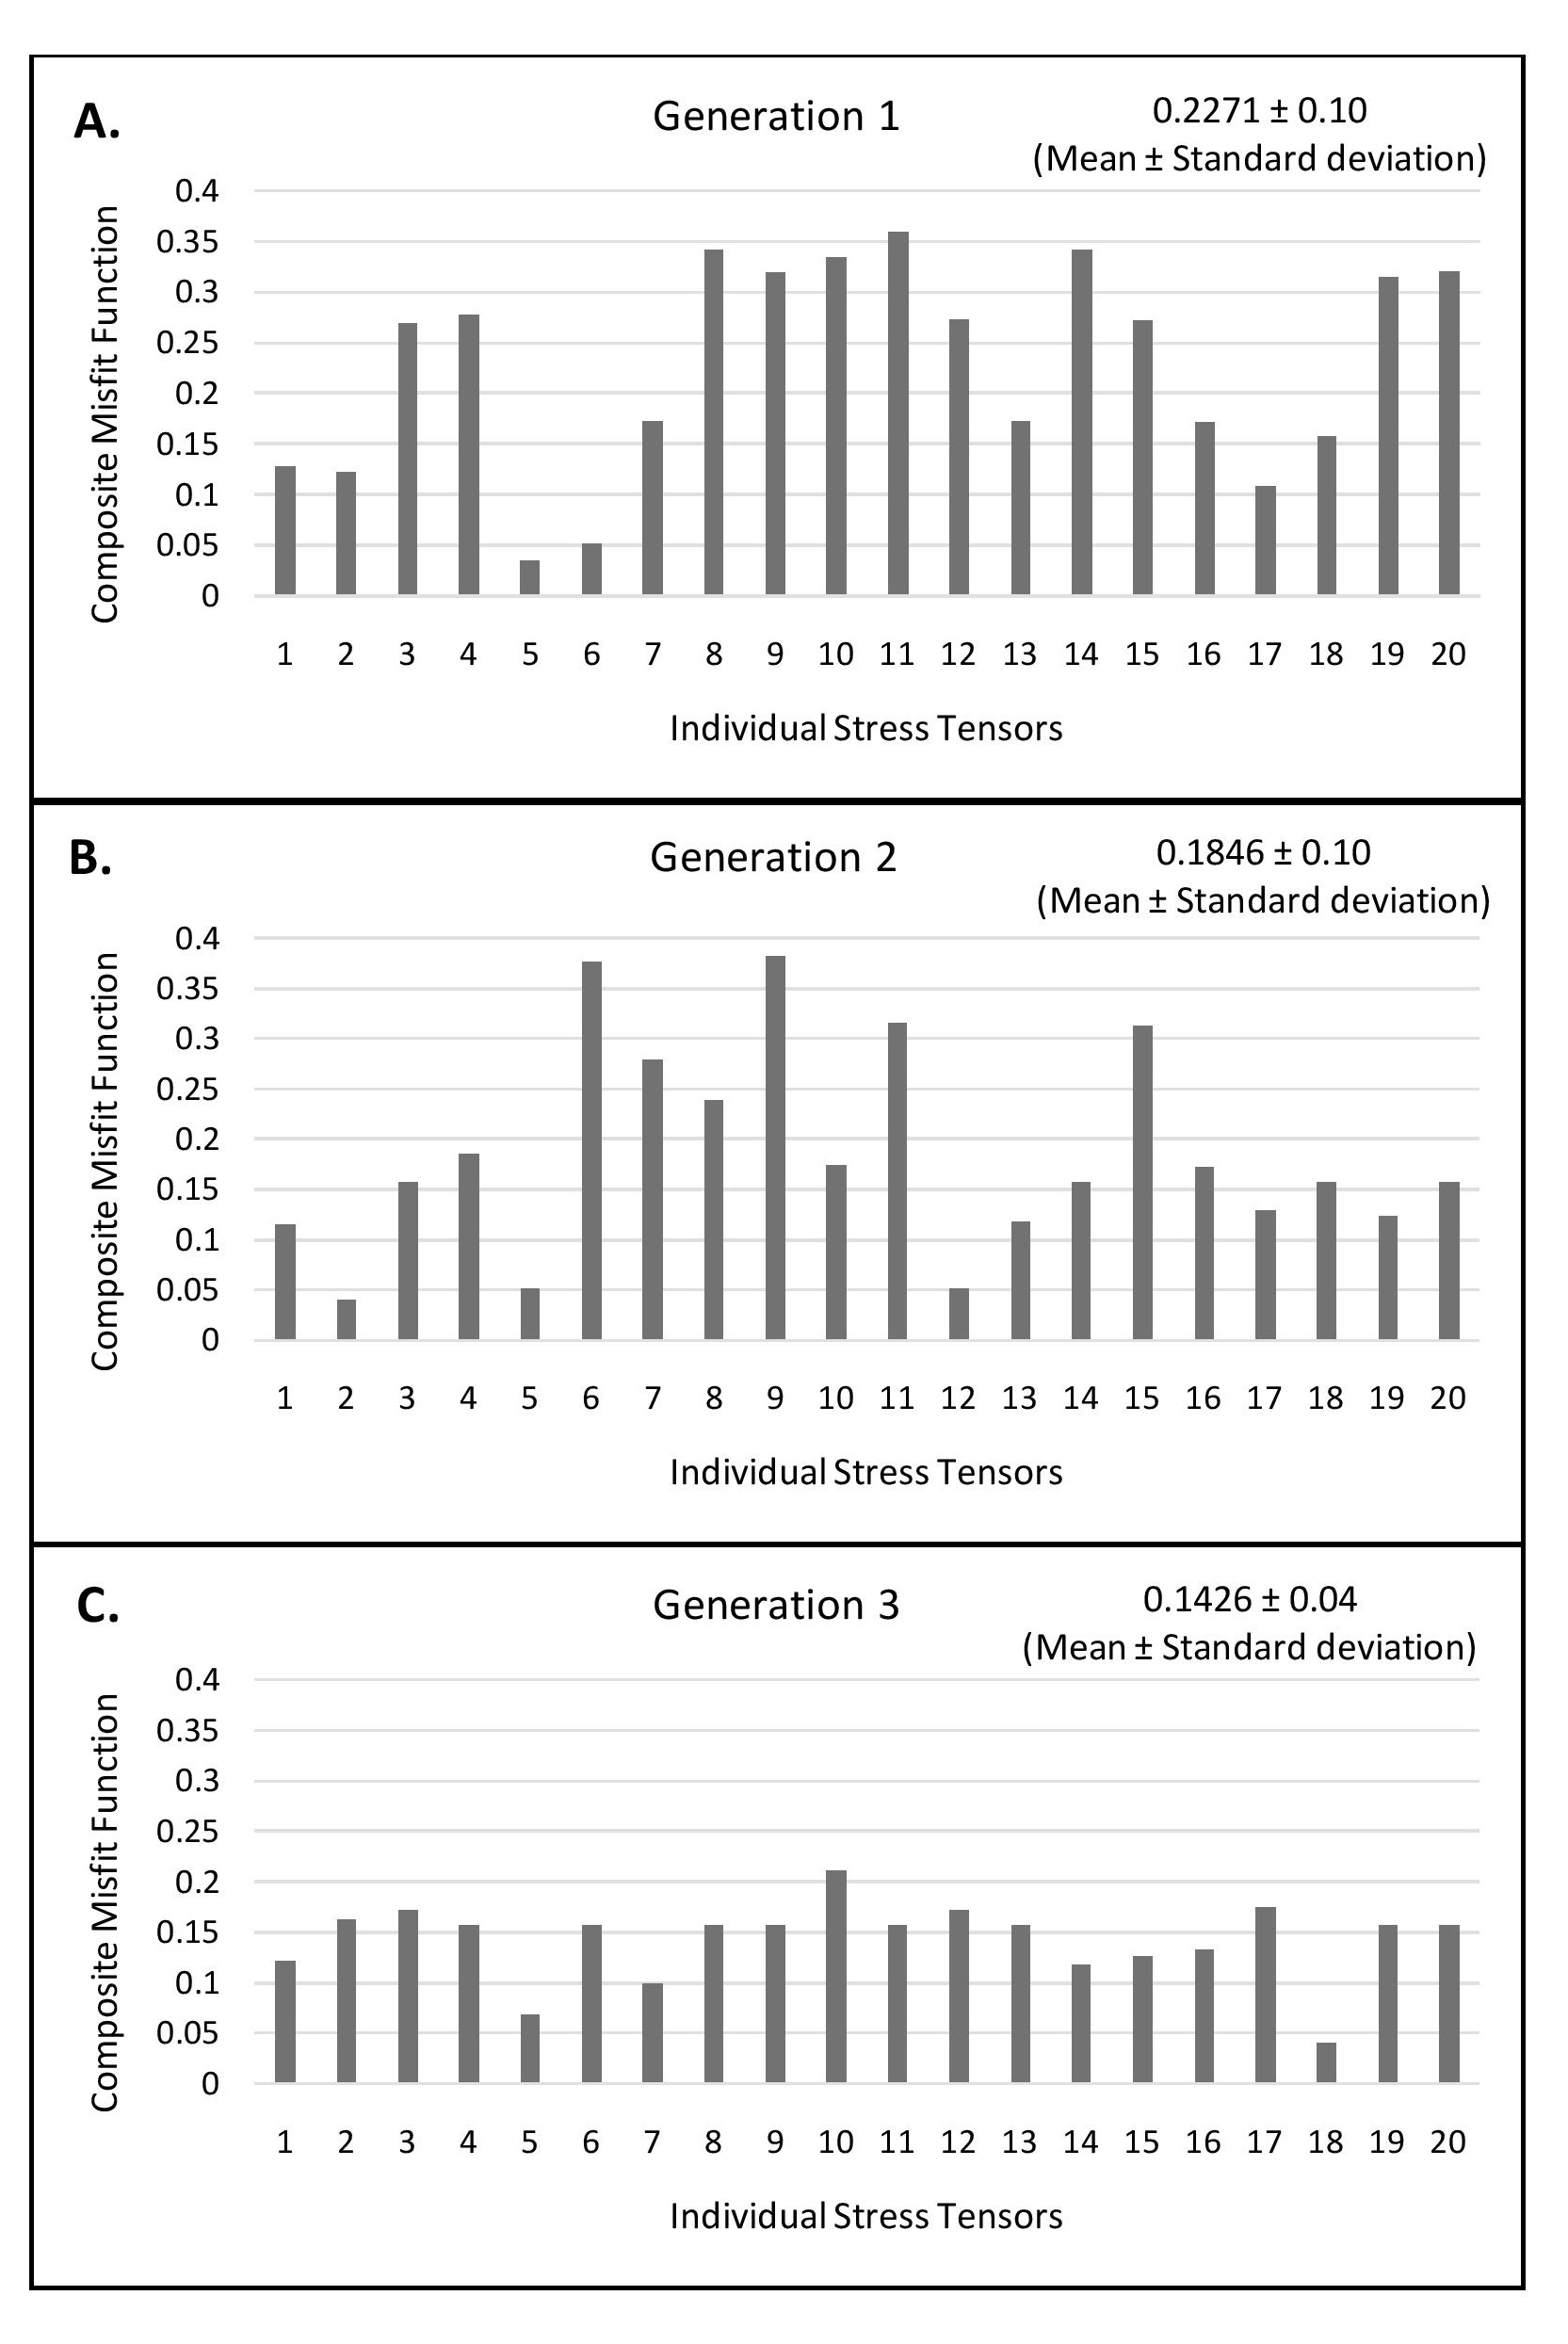
\includegraphics[scale = 1.0]{1}
\end{subfigure}
\end{figure}
\pagebreak
\begin{figure}[h!]
\ContinuedFloat
\begin{subfigure}{\textwidth}
    \centering
    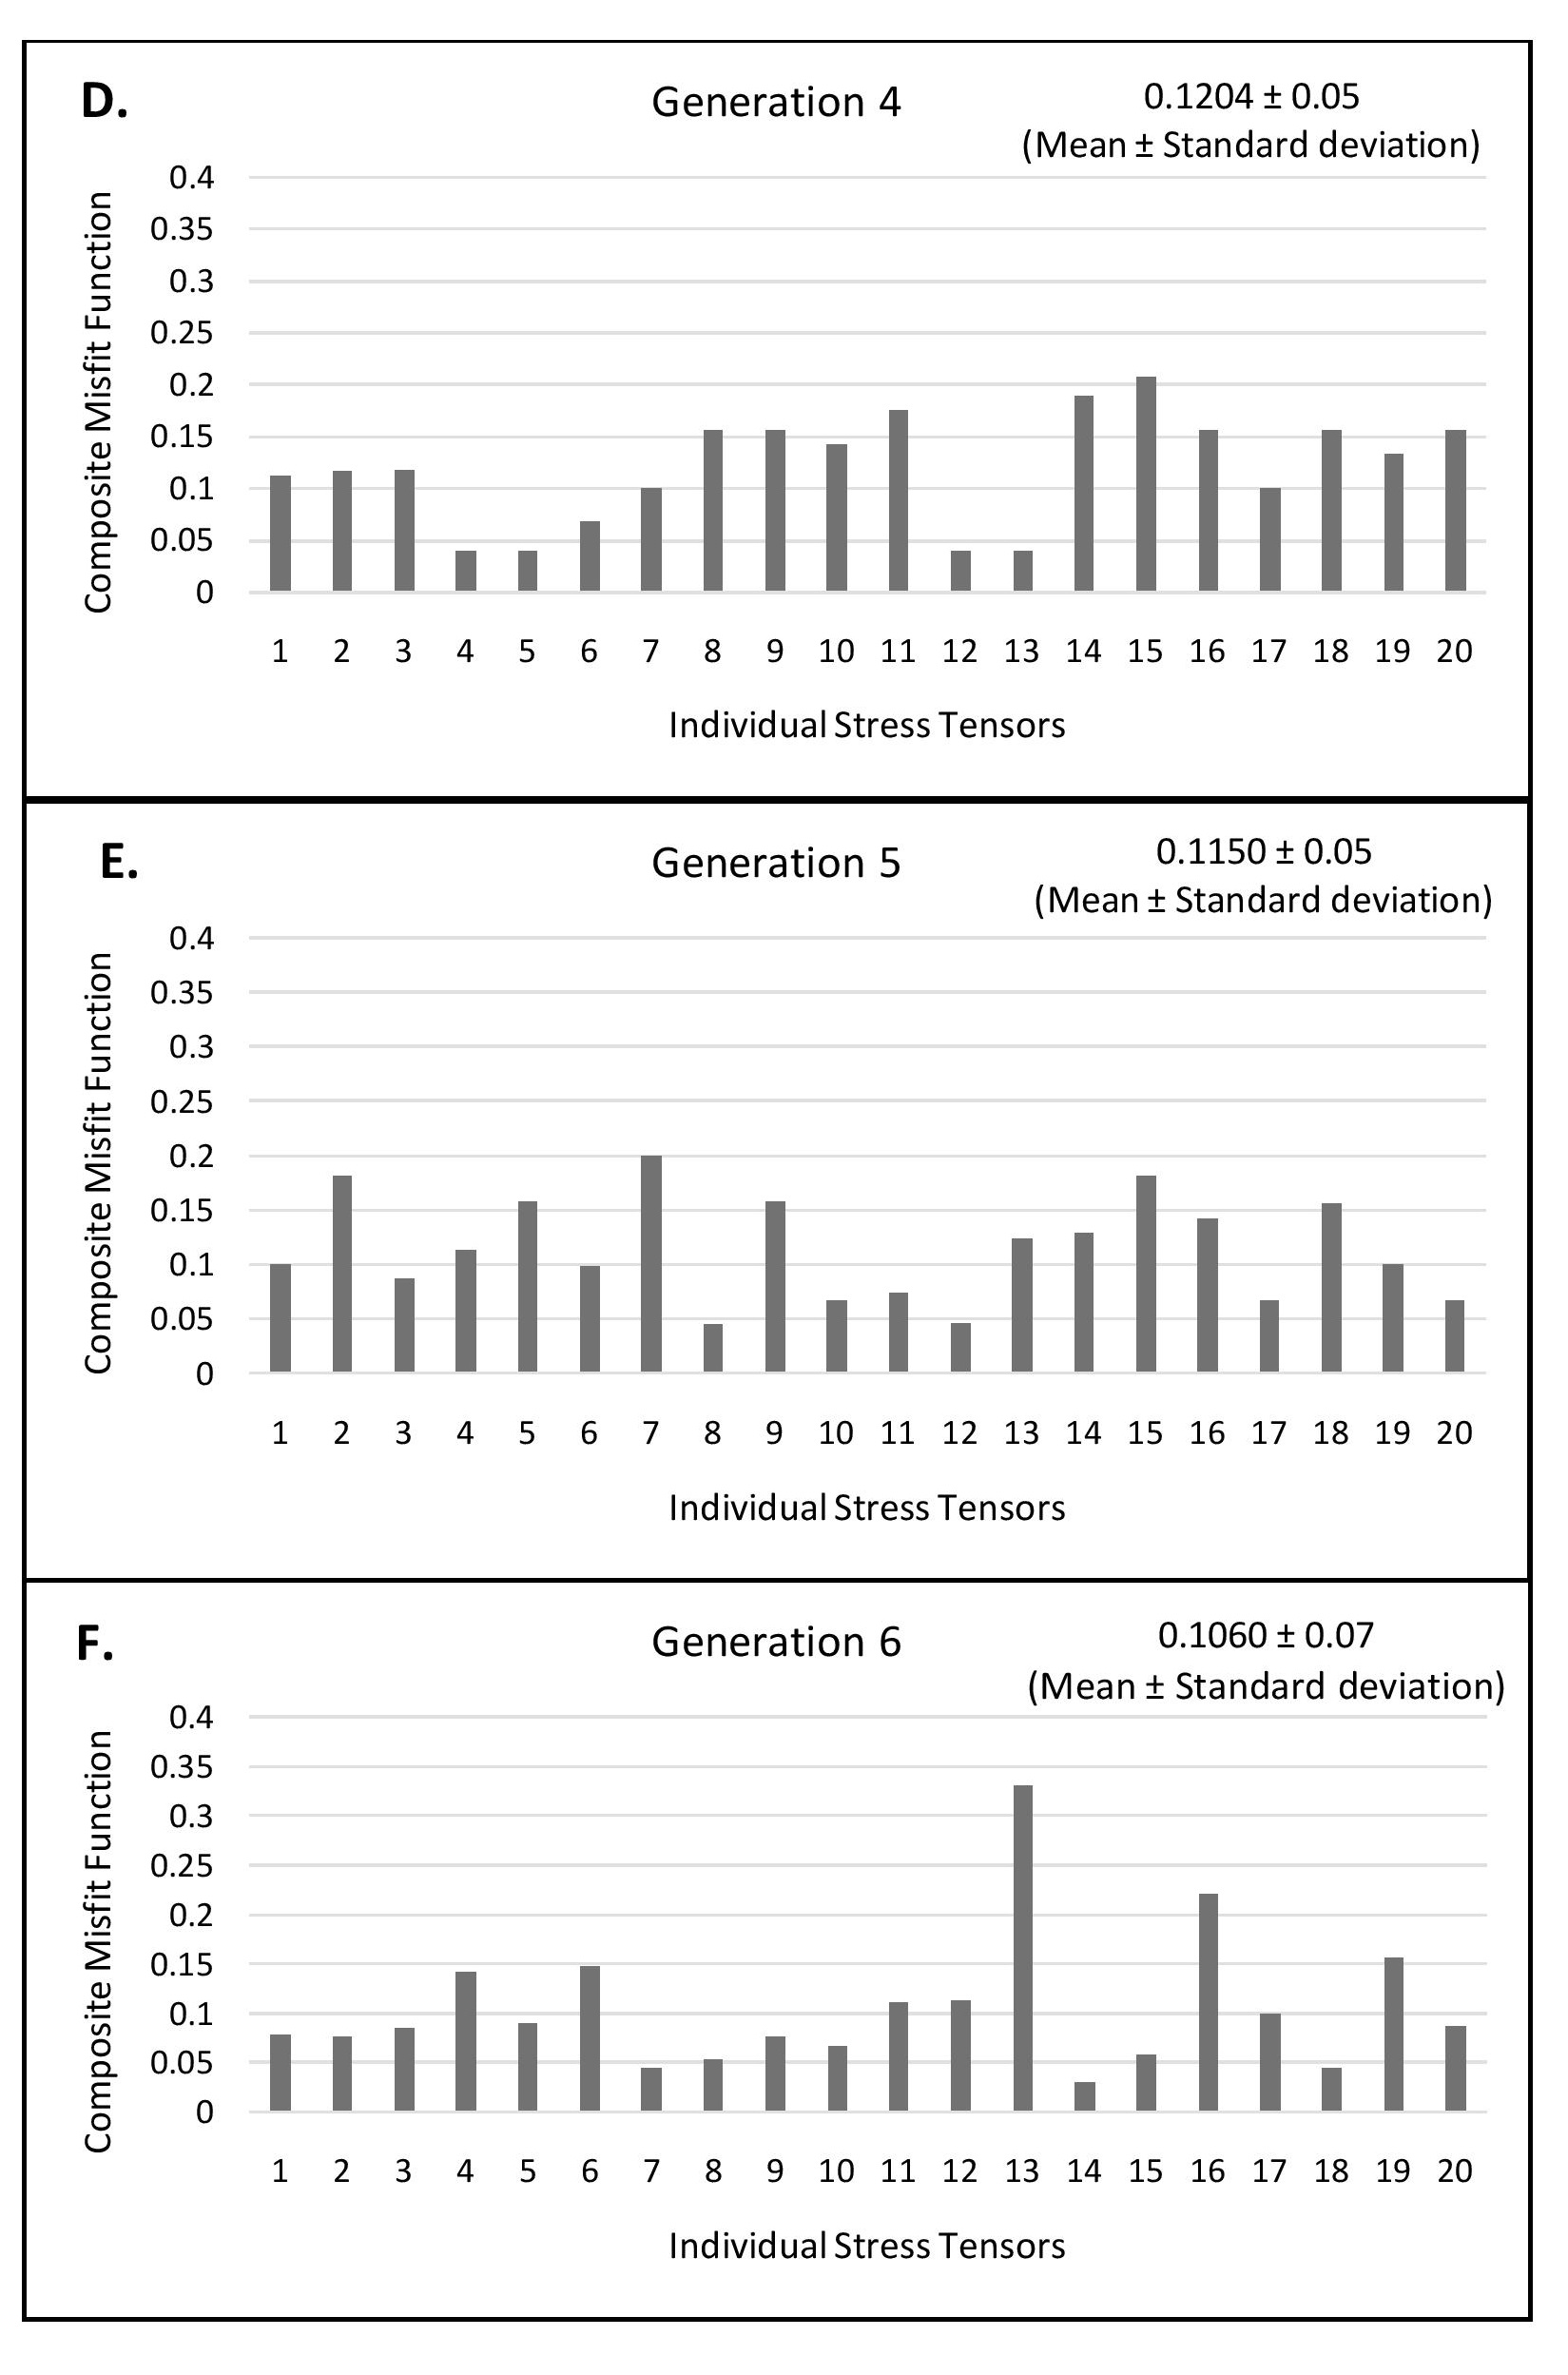
\includegraphics[scale = 1.0]{2}
\end{subfigure}
\end{figure}
\pagebreak
\begin{figure}[h!]
\ContinuedFloat
\begin{subfigure}{\textwidth}
    \centering
    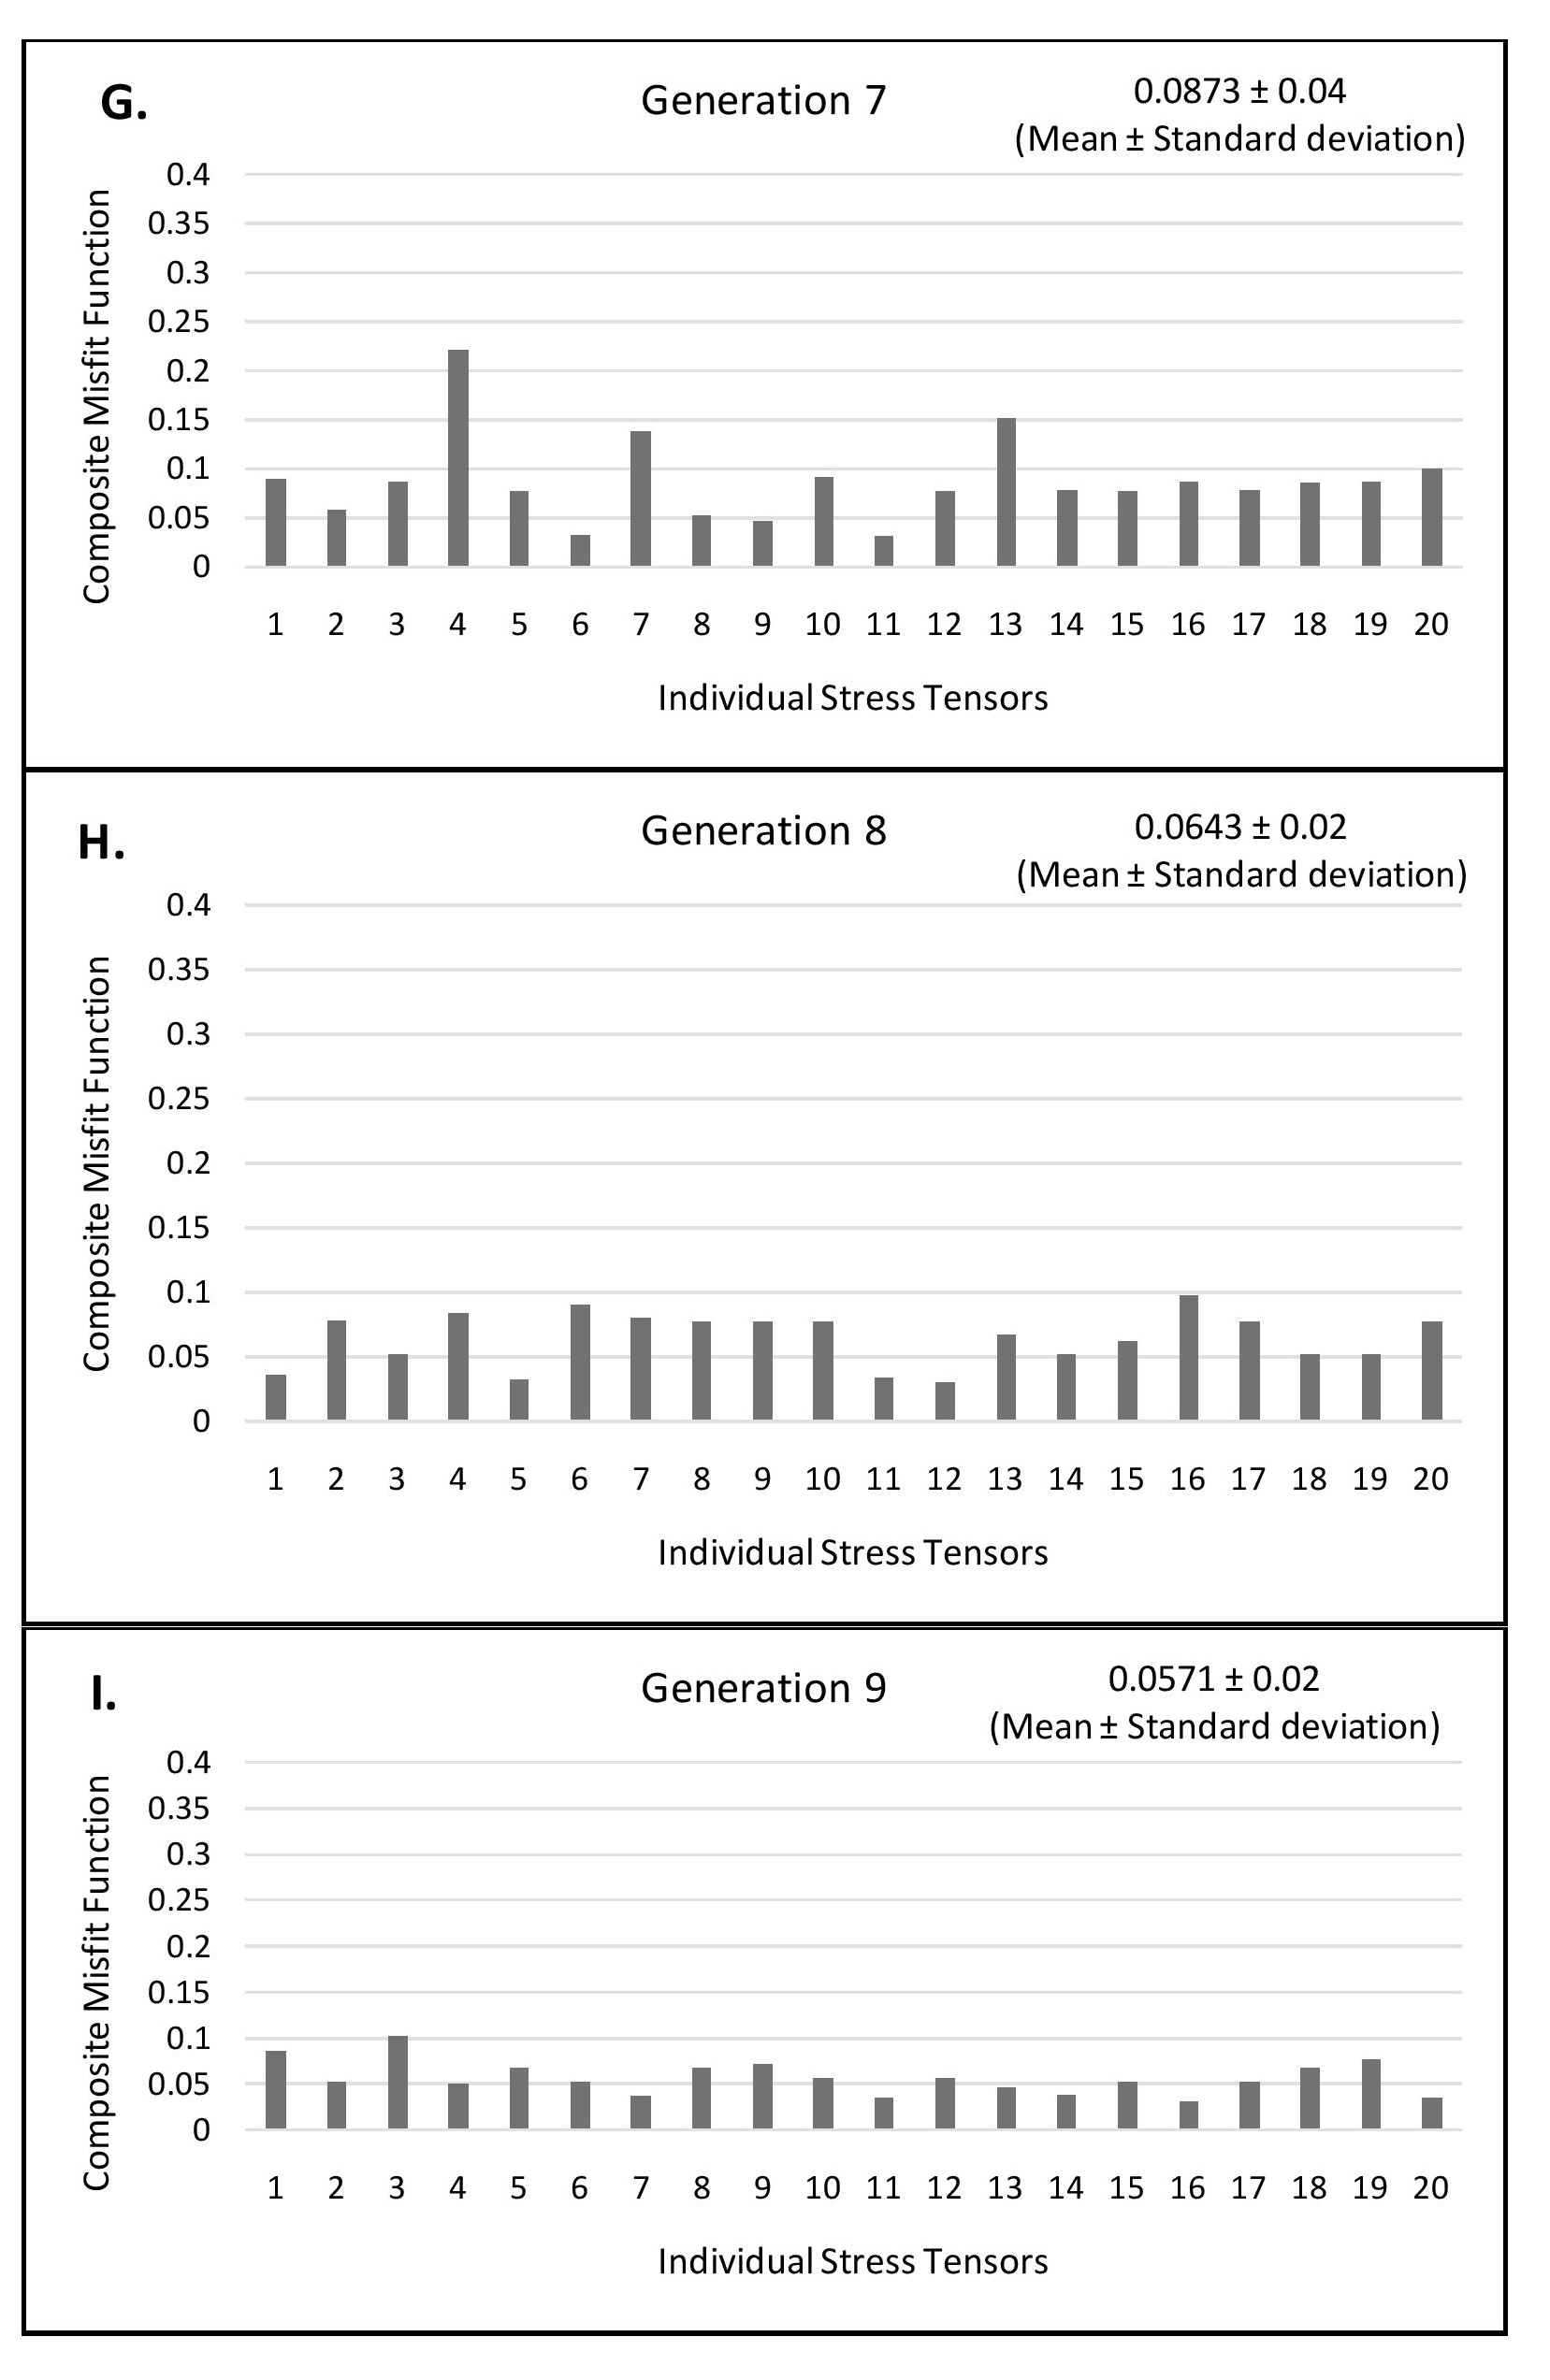
\includegraphics[scale = 1.0]{3}
\end{subfigure}
\end{figure}
\pagebreak
\begin{figure}[htb]
\ContinuedFloat
\begin{subfigure}{\textwidth}
    \centering
    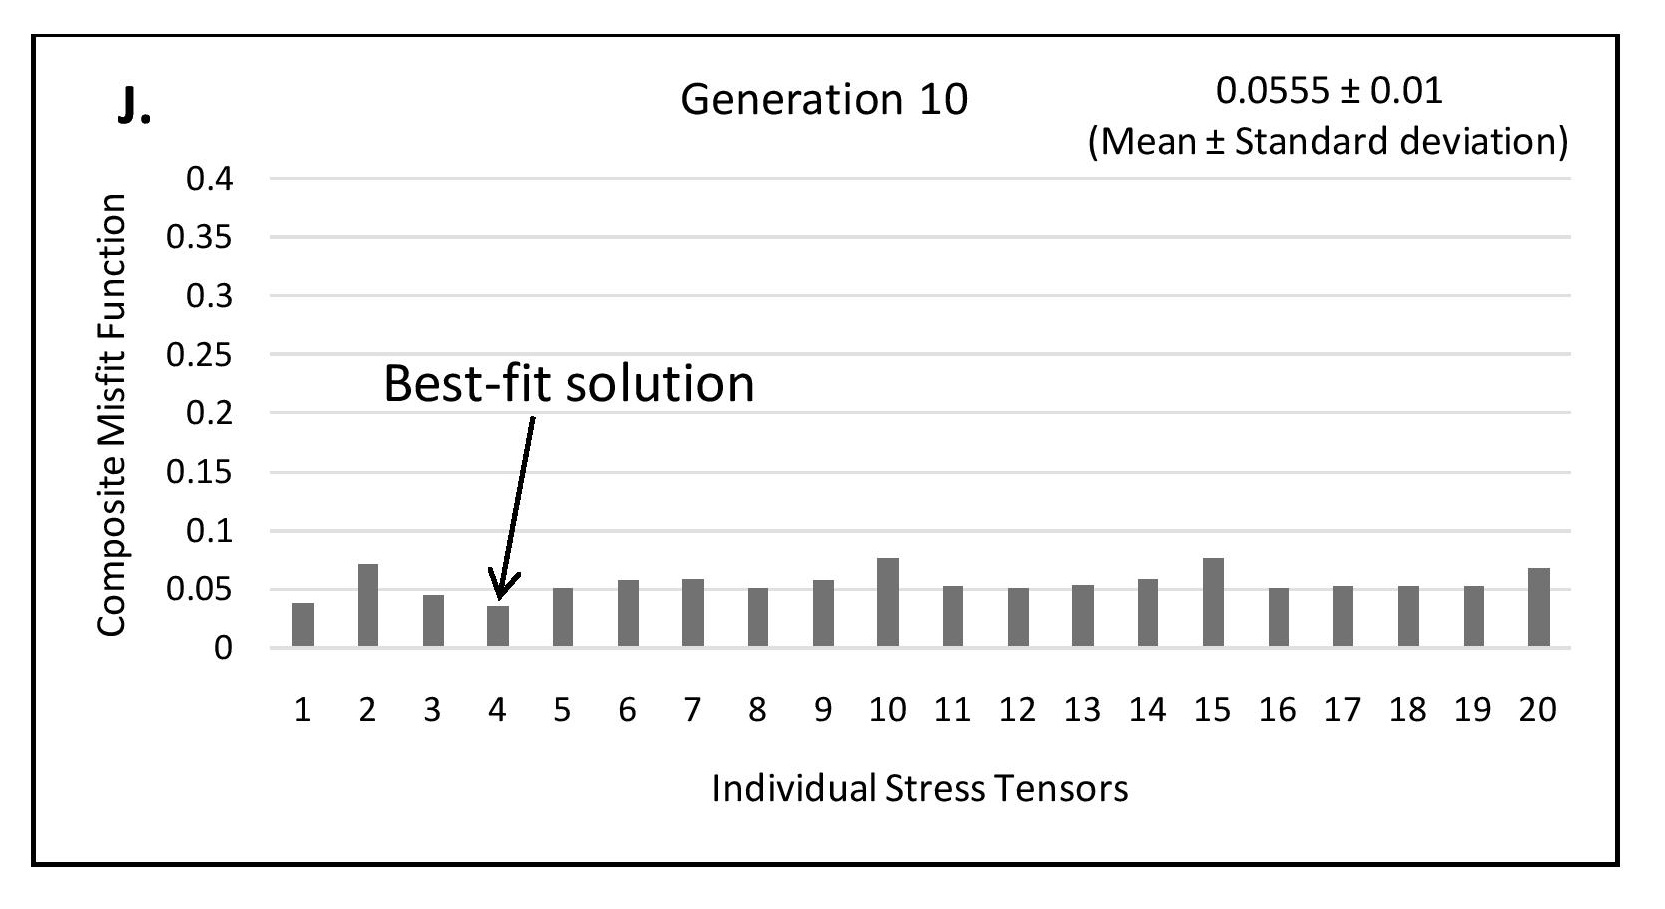
\includegraphics[scale = 1.0]{4}
\end{subfigure}
\caption{\textbf{A-J}: Composite misfit function for 10 iterations of the GA.}
\end{figure}


As the average misfit reduces, better individuals are produced in successive generations (Fig. 8:A-J). In the given population, the average misfit $\pm$ standard deviation reduce from $0.2271 \pm 0.10$ in the 1st generation to $0.0555 \pm 0.01$ in the 10th generation (Fig. 8:A-J). The 4th tensor in $10^{th}$ generation, having minimum composite misfit, is the optimum and required solution (Fig. 8:J).

\chapter*{Manuscripts Prepared}
\addcontentsline{toc}{chapter}{Manuscripts Prepared}
\lhead{\emph{Manuscripts}}
\thispagestyle{empty}
{
\setlength{\parindent}{0cm}

\textbf{Thakur, P.}, Srivastava, D. C., and Gupta, P. K., The Genetic Algorithm: a robust method for stress inversion. (Submitted to Journal of Structural Geology) 

\textbf{Thakur, P.}, Gupta, P. K., and Srivastava, D., C., Separation of polyphase fault-slip observations using genetic algorithm. (Manuscript in preparation)
}


\chapter*{References}
\addcontentsline{toc}{chapter}{References}
\lhead{\emph{References}}
\thispagestyle{empty}
%\begin{enumerate}
\footnotesize
{
\setlength{\parindent}{0cm}
\begin{hangparas}{.25in}{1}
    
    Anderson, E.M., 1951, The Dynamics of Faulting: Oliver \& Boyd, Edinburgh, p. 231–248.
    
    Angelier, J., 1975, Sur l’analyse de measures recueillies dans des sites failles: l’utilite d’une confrontation entre les methods dynamiques et cinematiques: Comptes Rendus de l’Academie des Sciences, Paris, v. D281, p. 1805–1808.
    
    Angelier, J., 1979, Determination of the mean principal directions of stresses for a given fault population: Tectonophysics, v. 56, p. T17–T26.
    
    Angelier, J., 1984, Tectonic analysis of fault slip data sets: Journal of Geophysical Research, v. 89, p. 5835–5848.
    
    Angelier, J., 1990, Inversion of field data in fault tectonics to obtain the regional stress—III. A new rapid direct inversion method by analytical means: Geophysical Journal International, v. 103, p. 363–376.
    Angelier, J., 1994. Fault slip analysis and palaeostress reconstruction, in Hancock, P.L., ed., Continental Deformation: Pergamon Press, Oxford, p. 53–100.

    Angelier, J., Tarantola, A., Valette, B., and Manoussis, S. 1982, Inversion of field data in fault tectonics to obtain the regional stress – I. Single phase fault populations: a new method of computing the stress tensor: Geophysical Journal of the Royal Astronomical Society, v. 69, p. 607–621.

    Barker, P., 1999, Genetic Algorithms and their use in Geophysical Problems, Ernest Orlando Lawrence Berkeley National Laboratory [PhD Thesis]: Berkeley, University of California, p. 61–66.

    Bishop, A., W., 1966, The strength of soils as engineering materials – 6th Rankine lectures: Geotechnique, v. 16, p. 91–130.

    Bott, M.H.P., 1959, The mechanics of oblique slip faulting: Geological Magazine, v. 96, p. 109–117.

    Byerlee, J.D., 1978, Friction of rocks: Pure and Applied Geophysics, v. 116, p. 615–626.

    Carey, E., and Brunier, B., 1974, Analyse théorique et numérique d'un modèle mécanique élémentaire appliqué à l'étude d'une population de failles: C. R. Academy of Science, Paris, D, v. 279, p. 891–894.

    Célérier, B., 1988, How much does slip on reactivated fault plane constrain the stress tensor?: Tectonics, v. 7, p.1257–1278.
    
    Celerier, B., Etchecopar, A., Bergerat, F., Vergely, P., Arthaud, F., and Laurent, P., 2012, Inferring stress from faulting: from early concepts to inverse methods: Tectonophysics, 581, 206-219.

    Chop, P., Y., Angelier, J., and Souffache, B., 1996, Distribution of angular misfits in fault-slip data: Journal of Structural Geology, v. 18, p. 1353–1367.

    Delvaux, D., and Sperner, B. 2003, Stress tensor inversion from fault kinematic indicators and focal mechanism data: the TENSOR program. In: new insights into Structural Interpretation and Modelling (D. Nieuwland Ed.): Geological Society, London, Special Publications, 212:75–100.

    Engelder, T., 1993, Stress regimes in the lithosphere: Princeton, NJ, Princeton University Press, 457 p.

    Etchecopar, A., Vasseur, G., and Daignieres, M., 1981, An inverse problem in microtectonics for the determination of stress tensors from fault striation analysis: Journal of Structural Geology v. 14, p. 1121–1131.
    
    Fry, N., 1999, Striated faults: visual appreciation of their constraint on possible paleostress tensors: Journal of Structural Geology, v. 21, p. 7-21. 

    Gephart, J.W., and Forsyth, D.W., 1984, An improved method for determining the regional stress tensor using earthquake focal mechanism data: application to the San Fernando earthquake sequence: Journal of Geophysical Research, v. 89, p. 9305–9320.

    Gerstoft, P., 1994, Inversion of seismoacoustic data using genetic algorithms and aposteriori probability distributions: The Journal of the Acoustical Society of America, v. 95, p. 770–782.

    Goldberg, D.E., 1989, GAs in Search, Optimization and Machine Learning: Kluwer Academic Publishers, Boston, MA, p. 1–40.
    
    Hansen, J. A., Bergh, S. G., Osmundsen, P. T., and Redfield, T. F., 2015. Stress inversion of heterogeneous fault-slip data with unknown slip sense: An objective function algorithm contouring method: Journal of Structural Geology, v. 70, p. 119-140.

    Hardebeck, J.L., and Hauksson, E., 2001, Stress orientations obtained from earthquake focal mechanisms: what are appropriate uncertainty estimates?: Bulletin of the Seismological Society of America, v. 91, p. 250–262.

    Hardcastle, K.C., and Hills, L.S., 1991, Brute3 and Select: Quickbasic 4 programs for determination of stress tensor configurations and separation of heterogeneous populations of fault-slip data: Computers \& Geosciences, v. 17, p. 23–43.

    Holland, J.H., 1975, Adaptation in Natural and Artificial Systems. Ann Arbor: University of Michigan Press, 183p.
    
    Kozak, A., 2008, Introduction to probability and statistics: applications for forestry and natural sciences: CABI, 2008.
    
    Liesa, C. L., and Lisle, R. J., 2004. Reliability of methods to separate stress tensors from heterogeneous fault-slip data: Journal of Structural Geology, v. 26, p. 559-572. 

    Lisle, R.J., and Srivastava, D.C., 2004, Test of the frictional reactivation theory for faults and validity of fault-slip analysis: Geology, v. 32, p. 569–572.
    
    Lisle, R.J., Orife, T.O., Arlegui, L., Liesa, C., and Srivastava, D.C., 2006, Favoured states of paleostress in the Earth’s crust: evidence from fault-slip data. Journal of Structural Geology v. 28, p. 1051–1066.
    
    Liu, Y., Wu, X., and Shen, Y., 2011, Automatic clustering using genetic algorithms: Applied Mathematics and computation, v. 281, p. 1267-1279.

    Michael, A., 1984, The determination of stress from slip data, faults and folds: Journal of Geophysical Research, v. 89, p. 11517–11526.
    
    Nemcok, M., and Lisle, R. J., 1995, A stress inversion procedure for polyphase fault/slip data sets: Journal of Structural Geology, v. 17, p. 1445-1453. 

    Nemcok, M., Kovac, D., and Lisle, R. J., 1999, A stress inversion procedure for polyphase calcite twin and fault-slip data sets: Journal of Structural Geology, v. 21, p. 597-611.
    
    Pollard, D., D., Saltzer, S., D., and Rubin, A., M., 1993, Stress inversion methods: are they based on faulty assumptions?: Journal of Structural Geology, v. 15, p. 1045–1054.
    
    Ray, A., and Srivastava, D. C., 2008, Non-linear least squares ellipse fitting using the genetic algorithm with applications to strain analysis: Journal of Structural Geology, v. 30, p. 1593–1602.

    Sambridge, M., and Drijkoningen, G., 1992, Genetic algorithms in seismic waveform inversion: Geophysical Journal International, v. 109, p. 323–342.

    Sen, M., Stoffa, P.L., 1995, Global Optimization Methods in Geophysical Inversion: Elsevier Science, B.V, p. 125–157.
    
    Shan, Y., Suen, H., and Lin, G., 2003, Separation of polyphase fault/slip data: an objective-function based on hard division: Journal of Structural Geology, v. 25, p. 829-840.

    Shan, Y., Li, Z., and Lin, G., 2004, A stress inversion procedure for automatic recognition of polyphase fault/slip data sets: Journal of Structural Geology, v. 26, p. 919-925. 

    Shan, Y., and Fry, N., 2005, A hierarchical cluster approach for forward separation of heterogeneous fault/slip data into subsets: Journal of Structural Geology, v. 27, p. 929-936. 

    Shan, Y., and Fry, N., 2006, The moment method used to infer stress from fault/slip data in sigma space: invalidity and modification: Journal of structural geology, v. 28, p. 1208-1213.  

    Shan, Y., Gong, F., Li, Z., and Lin, G., 2007, A grid-search inversion method looking for the best classification of polyhase fault/slip data: Tectonophysics, v. 433, p. 53-64. 

    Spang, J., H., 1972, Numerical method for dynamic analysis of calcite twin lamellae: Geological Society of America Bulletin, v. 83, p. 467–472.

    Wallace, R.E., 1951, Geometry of shearing stress and relation to faulting: Journal of Geology, v. 59, p. 118–130.
    
    Xu, P., 2004, Determination of regional stress tensors from fault–slip data: Geophysical Journal International, v. 157, p. 1316–1330.
    
    Yamaji, A., 2000, The multiple inverse method: a new technique to separate stresses from heterogeneous fault-slip data: Journal of Structural Geology, v. 22, p. 441-452.
    
    Yamaji, A., 2007, An Introduction to Tectonophysics: Theoretical Aspects of Structural Geology. Terrapub, Tokyo, p. 271–282.

    Yin, Z., M., and Ranalli, G., 1995, Estimation of frictional strength of faults from inversion of fault-slip data: a new method: Journal of Structural Geology, v. 17, p. 1327–1335.

    Zajac, B.J., and Stock, J.M., 1997, Using borehole breakouts to constrain the complete stress tensor: Results from the Sijan Deep Drilling Project and offshore Santa Maria Basin, California: Journal of Geophysical Research:, v 102, p. 10083–10100.

    Zang, A., and Stephansson, O., 2010, Stress Field of the Earth’s Crust: Springer, Amsterdam, 319 p.

\end{hangparas}
}


\end{document}